\documentclass{beamer}
% \usepackage{BioconductorSlides}

\usepackage[utf8]{inputenc}
\usepackage{graphicx}
%\usepackage[T1]{fontenc}
\usepackage{amsmath,amssymb,amsfonts,textcomp,setspace,graphicx,tikz,color}
\usepackage[absolute,overlay]{textpos}
  \setlength{\TPHorizModule}{1mm}
  \setlength{\TPVertModule}{1mm}
  
\AtBeginDocument{
\DefineVerbatimEnvironment{Sinput}{Verbatim} {xleftmargin=1em,fontsize=
\tiny}
\DefineVerbatimEnvironment{Soutput}{Verbatim}{xleftmargin=1em,fontsize=
\tiny}
\DefineVerbatimEnvironment{Scode}{Verbatim}{xleftmargin=1em,fontsize=
\tiny}
}

%%%%%%%%%%%%%%%%%%%%%%%%%%%%%%%%%%%%%%%%%%%%%%%%%%%%%%%%%%%%%%
%%%%%%%%%%%%   MODIFICAR AQUESTA SECCIÓ      %%%%%%%%%%%%%%%%%
%%%%%%%%%%%%%%%%%%%%%%%%%%%%%%%%%%%%%%%%%%%%%%%%%%%%%%%%%%%%%%
\title{Bioconductor packages for short read analyses}

\author{Alex S\'anchez}
\institute[UEB]{Unitat d'Estadística i Bioinformàtica (UEB)\\
  	}
\date{\today}
%%%%%%%%%%%%%%%%%%%%%%%%%%%%%%%%%%%%%%%%%%%%%%%%%%%%%%%%%%%%%%
%%%%%%%%%%%%%%%%%%%%%%%%%%%%%%%%%%%%%%%%%%%%%%%%%%%%%%%%%%%%%%
%%%%%%%%%%%%%%%%%%%%%%%%%%%%%%%%%%%%%%%%%%%%%%%%%%%%%%%%%%%%%%
\usetheme{Berkeley}
%itemize
\newcommand{\bit}{\begin{itemize}}
\newcommand{\eit}{\end{itemize}}

%enumerate
\newcommand{\ben}{\begin{enumerate}}
\newcommand{\een}{\end{enumerate}}

%Blue box
\newcommand{\bB}[1]{\begin{problock}{#1}}
\newcommand{\eB}{\end{problock}}

%Green box
\newcommand{\bG}[1]{\begin{exampleblock}{#1}}
\newcommand{\eG}{\end{exampleblock}}

%Red box
\newcommand{\bR}[1]{\begin{alertblock}{#1}}
\newcommand{\eR}{\end{alertblock}}

%colors
\definecolor{dB}{RGB}{80,13,138}
\definecolor{lB}{RGB}{153,0,153}

\definecolor{dG}{rgb}{0.00,0.50,0.00}
\definecolor{lG}{rgb}{0.71,0.81,0.69}

%custom blocks

\newenvironment<>{problock}[1]{%
  \begin{actionenv}#2%
      \def\insertblocktitle{#1}%
      \par%
      \mode<presentation>{%
       \setbeamercolor{block title}{fg=white,bg=Plum}
       \setbeamercolor{block body}{fg=black,bg=lightpurple}
       \setbeamercolor{itemize item}{fg=Plum}
       \setbeamertemplate{itemize item}[triangle]
     }%
      \usebeamertemplate{block begin}}
    {\par\usebeamertemplate{block end}\end{actionenv}}



\usepackage{Sweave}
\begin{document}
\Sconcordance{concordance:2.Bioconductor_BLAU.tex:2.Bioconductor_BLAU.Rnw:%
1 36 1 1 0 83 1 1 2 1 0 3 1 19 0 1 2 7 1 1 2 6 0 1 1 7 0 1 1 32 0 1 2 %
125 1 1 2 1 0 1 2 7 0 1 2 43 1 1 2 1 0 1 2 1 0 8 1 3 0 1 2 10 1 1 2 1 0 %
2 1 3 0 1 2 25 1 1 2 1 0 1 1 22 0 1 2 17 1 1 2 1 0 2 1 5 0 1 1 5 0 1 1 %
7 0 1 2 2 1 1 2 7 0 1 2 10 1 1 2 13 0 1 1 8 0 1 1 12 0 1 1 9 0 1 2 10 1 %
1 2 15 0 1 2 4 1 1 2 1 0 1 1 8 0 1 2 3 1 1 2 14 0 1 2 76 1 1 2 9 0 1 1 %
7 0 1 2 2 1 1 2 9 0 1 1 8 0 1 1 7 0 1 2 12 1 1 2 13 0 1 1 13 0 1 2 4 1 %
1 2 13 0 1 1 13 0 1 2 12 1 1 2 7 0 1 1 7 0 1 2 10 1 1 2 12 0 1 1 11 0 1 %
2 2 1 1 2 6 0 1 1 5 0 1 1 3 0 1 2 10 1 1 2 1 0 1 1 12 0 5 1 9 0 1 2 11 %
1 1 2 24 0 1 2 10 1 1 2 1 0 2 1 6 0 1 2 2 1 1 2 9 0 1 1 9 0 1 2 34 1 1 %
2 1 0 1 1 11 0 1 2 21 1 1 2 7 0 1 5 24 1 1 2 1 0 1 1 5 0 1 1 7 0 1 2 2 %
1 1 2 8 0 1 2 19 1 1 2 1 0 1 1 7 0 1 2 10 1 1 2 1 0 1 1 14 0 1 4 12 1 1 %
2 1 0 2 1 17 0 1 2 7 1 1 2 26 0 1 6 12 1 1 2 11 0 1 1 1 2 6 0 1 4 8 1 1 %
2 58 0 1 6 101 1 1 2 1 0 1 1 11 0 2 1 3 0 1 2 7 1 1 2 1 0 1 1 24 0 1 2 %
23 1 1 2 1 0 2 1 41 0 1 3 52 1 1 2 1 0 2 1 18 0 2 1 12 0 1 2 12 1 1 6 8 %
0 1 2 123 1 1 4 3 0 1 1 15 0 1 2 2 1 1 2 10 0 1 2 45 1 1 2 17 0 1 3 15 %
1 1 2 15 0 1 1 15 0 1 2 7 1 1 2 16 0 1 2 2 1 1 2 16 0 1 2 14 1 1 2 1 0 %
1 1 13 0 1 2 55 1 1 2 1 0 1 1 8 0 1 2 20 1 1 2 12 0 1 2 53 1 1 2 1 0 7 %
1 21 0 1 2 8 1 1 2 16 0 1 1 4 0 1 3 52 1 1 2 1 0 1 1 19 0 1 2 13 1 1 2 %
20 0 1 2 24 1 1 2 30 0 1 2 12 1 1 2 1 0 2 1 11 0 1 1 13 0 1 2 12 1 1 2 %
1 0 1 1 12 0 1 2 11 1 1 2 15 0 1 1 13 0 1 2 11 1 1 2 1 0 1 1 5 0 1 1 5 %
0 2 1 5 0 1 1 15 0 1 3 14 1 1 4 6 0 1 2 6 1 1 3 64 0 1 2 12 1 1 2 1 0 1 %
1 10 0 5 1 4 0 1 2 84 1 1 8 7 0 1 3 1 0 1 1 1 2 1 0 1 16 16 0 1 2 73 1}


\begin{frame}[plain]
%\addtocounter{totalframenumber}{-1}
\titlepage
\end{frame}

\begin{frame}[Frame 1]
\addtocounter{framenumber}{-1}
\frametitle{Table of Contents}
\tableofcontents
\end{frame}

%%%%%%%%%%%%%%%%%%%%%%%%%%%%%%%%%%%%%%%%%%%%%%%%%%%%%%%%%%%%%%%%%%%%%%%%%
%%%%%%%%%%%%      MODIFICAR A PARTIR D'AQUI       %%%%%%%%%%%%%%%%%%%%%%%
%%%%%%%%%%%%%%%%%%%%%%%%%%%%%%%%%%%%%%%%%%%%%%%%%%%%%%%%%%%%%%%%%%%%%%%%%

\section{General Information}

\subsection{Objectives}

\begin{frame}
\frametitle{Foreword}
  \bit
      \item The ``core'' packages for integrating NGS data anlysis represents a massive structure.
      \item It is under very active development and often different ways exist to achieve one goal.
	      \bit
	          \item \emph{e.g RangedData vs. GRanges}
	      \eit
      \item The trunk of this core starts to reach maturity and redundant branches might be pruned.
  \eit
\end{frame}


%--------------------------------------------------------------------------------------------------------------------------------

\begin{frame}
\frametitle{ALM}
 \bit
      \item Introduce all the necessary packages to perfom the QA and the pre-processin of NGS rawdata:
        \bit
	          \item\textbf{biomRt}
	          \item\textbf{rtracklayer}
	          \item\textbf{Biostrings}
	          \item\textbf{BSgenome}
	          \item\textbf{GenomicFeatures}
	          \item\textbf{GenomicRanges}
	          \item\textbf{IRanges}
	          \item\textbf{Rsamtools}
	          \item\textbf{ShortRead}  
        \eit
 \eit
\end{frame}

%--------------------------------------------------------------------------------------------------------------------------------

\begin{frame}
\frametitle{Before we ``really'' start: the Classes in R}
 \bit
      \item Two kinds: S3 and S4
        \bit
	          \item S3 are old and informal, setting the class attribute is enough to ``convert'' an object into a class
	          \item S4 is an attempt at making R more object oriented
	            \bit
		              \item they have specific definitions
		              \item they define ``fields'' called ``\textbf{slots}''
		              \item they can inherit and be inherited from
		              \item they can have prototypes, validators
		              \item they can be virtual
		              \item etc.
	            \eit
	          \item Most of the classes described here are of S4 type, except when backward compatibility with the R core required otherwise
	          \item More information can be foun in the R help page: ?classRepresentation
       \eit
 \eit
\end{frame}

%--------------------------------------------------------------------------------------------------------------------------------

\begin{frame}[fragile]
\frametitle{Methods to browse S4 classes}
(Load the IRanges library to run the following example)
    \begin{uncoverenv}
\begin{Schunk}
\begin{Sinput}
> require(IRanges)
> ?Classes
> ?Methods
> getClass("RleList")
\end{Sinput}
\begin{Soutput}
Virtual Class "RleList" [package "IRanges"]

Slots:
                                                      
Name:      elementType elementMetadata        metadata
Class:       character DataTableORNULL            list

Extends: 
Class "AtomicList", directly
Class "List", by class "AtomicList", distance 2
Class "Vector", by class "AtomicList", distance 3
Class "Annotated", by class "AtomicList", distance 4

Known Subclasses: "RleViews", "CompressedRleList", "SimpleRleList"
\end{Soutput}
\end{Schunk}
    \end{uncoverenv}
\end{frame}

%--------------------------------------------------------------------------------------------------------------------------------

\begin{frame}[fragile]
\frametitle{Methods to browse S4 classes}
 \begin{uncoverenv}
\begin{Schunk}
\begin{Sinput}
> names(completeSubclasses(getClass("RleList")))
\end{Sinput}
\begin{Soutput}
[1] "RleViews"          "CompressedRleList" "SimpleRleList"    
\end{Soutput}
\begin{Sinput}
> head(showMethods(classes="RleList",printTo=FALSE))
\end{Sinput}
\begin{Soutput}
[1] ""                              "Function \"activeView\":"     
[3] " <not an S4 generic function>" ""                             
[5] "Function \"activeView<-\":"    " <not an S4 generic function>"
\end{Soutput}
\begin{Sinput}
> showMethods("values",includeDefs=TRUE)
\end{Sinput}
\begin{Soutput}
Function: values (package IRanges)
x="QASummary"
function (x, ...) 
{
    x@values
}


x="RangedData"
function (x, ...) 
{
    .local <- function (x) 
    x@values
    .local(x, ...)
}


x="SummarizedExperiment"
function (x, ...) 
{
    values(rowData(x), ...)
}


x="Vector"
function (x, ...) 
elementMetadata(x, ...)
\end{Soutput}
\end{Schunk}
  \end{uncoverenv}
\end{frame}

%--------------------------------------------------------------------------------------------------------------------------------

\begin{frame}
\frametitle{Packages dependencies}
 \bit
    \item Sometimes packages define the same function resulting in one of the function to be inaccessible anymore.
    \item When this happens, one needs to contact the packages authors for them to find an appropiate solution
    \item In the meanwhile, the hack described on the next slides might help
    \item load the GenomicRanges and the genomeIntervals in that order
 \eit
\end{frame}

%--------------------------------------------------------------------------------------------------------------------------------

\begin{frame}
\frametitle{Packages dependencies}
 \bit
    \item For the purpose og the example it is not necessary to 
    understand the actual obects taht are created. We'll come back to them later.
    \item Create the necessary object
      \bit
	  \item \small{grngs $<-$ GRanges (seqnames=c(``chr1'',``chr2'',``ch31''), 
	  ranges=IRanges(start=c(3,4,1),end=c(7,5,3)),s
	  trand=c(``+'',``+'',``\--''), seqlegths=c(``chr1''=24,``chr2''=18))}
      \eit
 \eit
\end{frame}

%--------------------------------------------------------------------------------------------------------------------------------

\begin{frame}
\frametitle{Bottom - up approach}
\begin{figure}[ht]
\centering
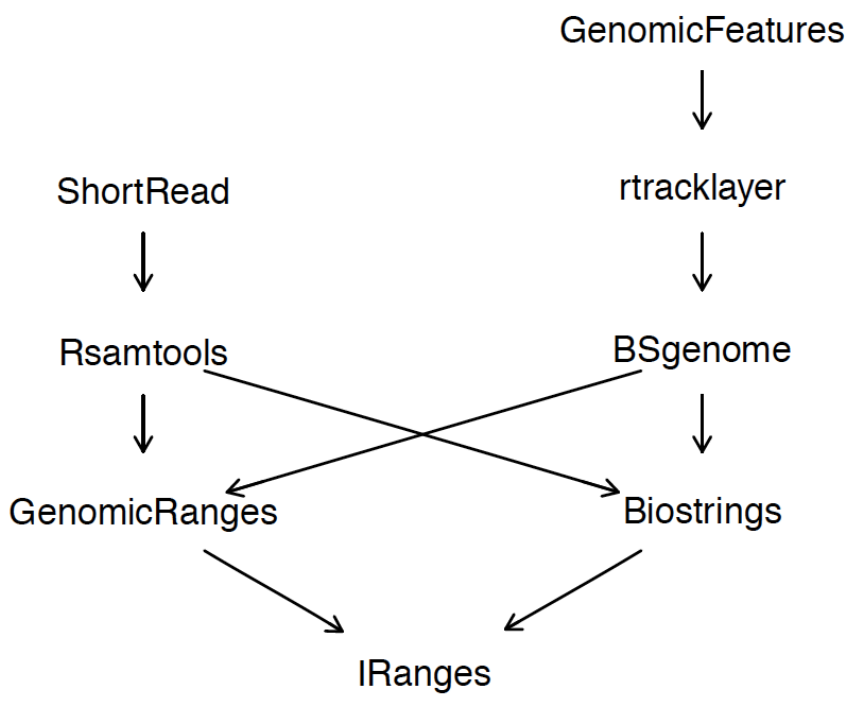
\includegraphics[width=80mm]{diagramas/Seleccio_001.png}
\end{figure}
\end{frame}

%--------------------------------------------------------------------------------------------------------------------------------

\begin{frame}
\frametitle{Infrastructure package}
 \bit
      \item \textbf{IRanges}
        \bit
	          \item Long sequences, compressed and pointer referenced
	          \item \textbf{Views} on long sequences
	          \item Integer overlap tppñs; e.g. interval overlap
	          \item Used to define genomic intervals (i.e. RangedData)
        \eit
      \item \textbf{GenomicRanges} \hspace{4.1cm} \fbox{ Recent }
        \bit
	          \item IRanges extension 
	          \item Adds discontiguous genomic interval sets (useful for gapped alignments)
        \eit
      \item \textbf{genomeIntervals} \hspace{4cm} \fbox{ Not Core}
        \bit
	          \item Very similar to IRanges  
	          \item Extremely efficient at interval calculations; e.g. interval overlap
        \eit
 \eit
\end{frame}

%--------------------------------------------------------------------------------------------------------------------------------

\begin{frame}
\frametitle{Infrastructure Views}
 \bit
    \item Issue
      \bit
	  \item DNA sequences can be very large (think of the human genome)
	  \item Duplicating them in memory is contra-efficient
      \eit
     \item Therefore the views!
      \bit
	  \item Views is yet another IRanges class
	    \bit
		      \item a virtual class for storin set of views (~pointers) on a single Sequence object
		      \item avaliable as RleViews, XStringViews, XIntegerViews, XStringSetViews, etc.
		      \item it stores the sequence using a ``pass-by-reference'' semantic and associatesranges to select the subsequences
	    \eit
      \eit
 \eit
\end{frame}

%--------------------------------------------------------------------------------------------------------------------------------

\begin{frame}
\frametitle{Infrastructure Running Length Encodings (RLEs)}
 \bit
    \item Issue
      \bit
	  \item Again, memory is the limit. holding a  coverage vector at a single bp resolution is inefficient.
      \eit
     \item Therefore the concept of RLEs
      \bit
	  \item a common compression technique for piecewise constant data
	    \bit
		\item 0 0 0 1 1 1 2 2 3 3 3 ... can be compressed in
		\item 0(3), 1(3), 2(2), 3(3),...
	    \eit
	   \item it couples values e.g. 0 with a run length i.e. 3
	   \item Can be partitioned into RleList, e.g. for storing the coverage of different chromosomes
      \eit
 \eit
\end{frame}

%--------------------------------------------------------------------------------------------------------------------------------

\begin{frame}[fragile]
\frametitle{Infrastructure methods}
 \bit
    \item get the metods for the Rle S4 class
      \bit
	  \item f.list$<-$showMethods(classes=``Rle'', printTo=FALSE) 
      \eit
     \item process the result to extract the function name
      \bit
	  \item sapply(strsplit(f.list[grep(``Function'',f.list,''), function(l){gsub('\:',``,l[[2]])}
      \eit
 \eit
\bB{ \textbf{\emph{This return 111 methods!}} }
      \begin{uncoverenv}
\begin{Schunk}
\begin{Sinput}
> f.list<-showMethods(classes="Rle", printTo=FALSE)
> length(sapply(strsplit( f.list[grep("Function",
+   f.list)],' '),function(l){gsub('\"|:','',l[[2]])}))
\end{Sinput}
\begin{Soutput}
[1] 340
\end{Soutput}
\end{Schunk}
 \end{uncoverenv}
    \eB
\end{frame}

%--------------------------------------------------------------------------------------------------------------------------------

\begin{frame}
\frametitle{Infrastructure methods, some examples}
 \bit
    \item \textbf{Arithmetic}  $+,-,*,^,\%\%,\% /\%,/$
    \item \textbf{Compare}
    $==,>,<,!=,<=,>=$
    \item \textbf{Logic}
    $\& ,| $
    \item \textbf{Math}
    abs, sign, sqrt, ceiling, floor, trunc, cummax, cummin, cumprod, cumsum, log, log10, log2, log1p, acos, acosh, asin, asinh,...
    \item \textbf{Math2}
    round,signif
    \item \textbf{Summmary}
    max, min, range, prod, sum, any, all
 \eit
\end{frame}

%--------------------------------------------------------------------------------------------------------------------------------

\begin{frame}
\frametitle{Looks intimidating}
 \bit
    \item Still the point is:
      \bit
	        \item whenever you think about a functionality, it probably already exists.
      \eit
 \eit

\end{frame}

%--------------------------------------------------------------------------------------------------------------------------------

\begin{frame}[fragile]
\frametitle{Example 1: coverage}
  \bit
      \item Coverage calculation
  \eit
  \begin{uncoverenv}
\begin{Schunk}
\begin{Sinput}
> require("ShortRead")
> fl<-system.file("extdata","GSM424494_wt_G2_orc_chip_rep1_S288C_14.mapview.txt.gz",
+                 package="EatonEtAlChiPseq")
> aln<-readAligned(fl,type="MAQMapview")
> cover<-coverage(aln);cover
> cover[["S288C_14"]]
> head(runValue(cover[["S288C_14"]]))
> as.integer(cover[["S288C_14"]])
> smoothCover<-round(runmean(cover,75,endrule="constant"))
> class(smoothCover)
> smoothCover
\end{Sinput}
\end{Schunk}
 \end{uncoverenv}
\end{frame}

%--------------------------------------------------------------------------------------------------------------------------------

\begin{frame}[fragile]
\frametitle{Example 2: slice}
  \bit
      \item Finding wide regions with elevated coverage
  \eit
  \begin{uncoverenv}
\begin{Schunk}
\begin{Sinput}
> islands<-slice(smoothCover,lower=10)
> islandsWithWidePeaks<- islands[vienMaxs(islands)>=20L &width(islands)>=500L]
> islandsWithWidePeaks
\end{Sinput}
\end{Schunk}
 \end{uncoverenv}
  
\end{frame}

%--------------------------------------------------------------------------------------------------------------------------------

\begin{frame}
\frametitle{What comes on top of IRanges}
  \bit
      \item We've ``covered'' \textbf{IRanges} and it's low level capabilities.
      \item Still, High Throughput methods in biology, especially sequencing, are more about sequenes than maths.
      \item Therefor the \textbf{Biostrings} package, build on top of IRanges
        \begin{figure}[ht]
              \centering
              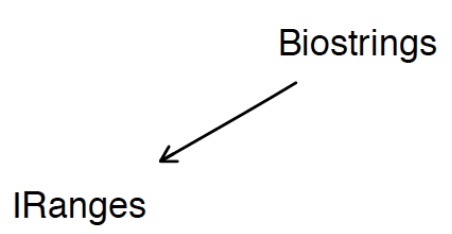
\includegraphics[width=50mm]{diagramas/Seleccio_004.png}
        \end{figure}
  \eit
\end{frame}

%--------------------------------------------------------------------------------------------------------------------------------

\begin{frame}[fragile]
\frametitle{Biostrings}
  \bit
      \item \small{All the classes in that package derivers from the XString class}
        \begin{uncoverenv}
\begin{Schunk}
\begin{Sinput}
> require(Biostrings)
> getClass("XString")
\end{Sinput}
\begin{Soutput}
Virtual Class "XString" [package "Biostrings"]

Slots:
                                                                      
Name:           shared          offset          length elementMetadata
Class:       SharedRaw         integer         integer DataTableORNULL
                      
Name:         metadata
Class:            list

Extends: 
Class "XRaw", directly
Class "XVector", by class "XRaw", distance 2
Class "Vector", by class "XRaw", distance 3
Class "Annotated", by class "XRaw", distance 4

Known Subclasses: "BString", "DNAString", "RNAString", "AAString"
\end{Soutput}
\end{Schunk}
        \end{uncoverenv}
      \item There are 4 subclasses:
        \bit
            \item \small{\textbf{BString}: store strings without alphabet}
            \item \small{\textbf{DNAString}: store strings with an DNA alphabet}
            \item \small{\textbf{RNAString}: store strings with an RNA alphabet}
            \item \small{\textbf{AAString}: store strings with an Amino Acid alphabet}
        \eit
  \eit
\end{frame}

%--------------------------------------------------------------------------------------------------------------------------------

\begin{frame}[fragile]
\frametitle{An DNAString example}
  \bit
      \item The \textbf{Biostring} package contains many example datasets
            \begin{uncoverenv}
\begin{Schunk}
\begin{Sinput}
> data(package="Biostrings")
> data(yeastSEQCHR1)
> class(yeastSEQCHR1)
\end{Sinput}
\begin{Soutput}
[1] "character"
\end{Soutput}
\begin{Sinput}
> nchar(yeastSEQCHR1)
\end{Sinput}
\begin{Soutput}
[1] 230208
\end{Soutput}
\begin{Sinput}
> DNAString(yeastSEQCHR1)
\end{Sinput}
\begin{Soutput}
  230208-letter "DNAString" instance
seq: CCACACCACACCCACACACCCACACACCACACCACA...GGTGTGTGGGTGTGGTGTGGGTGTGGTGTGTGTGGG
\end{Soutput}
\end{Schunk}
            \end{uncoverenv}
      \item The obtained DNAString is defined by the DNA alphabet
            \begin{uncoverenv}
\begin{Schunk}
\begin{Sinput}
> alphabet(DNAString(yeastSEQCHR1))
\end{Sinput}
\begin{Soutput}
 [1] "A" "C" "G" "T" "M" "R" "W" "S" "Y" "K" "V" "H" "D" "B" "N" "-" "+" "."
\end{Soutput}
\end{Schunk}
            \end{uncoverenv}
  \eit
\end{frame}

%--------------------------------------------------------------------------------------------------------------------------------

\begin{frame}[fragile]
\frametitle{The alphabets}
  \bit
      \item The \textbf{Biostring} package implements the possible alphabets
        \begin{uncoverenv}
\begin{Schunk}
\begin{Sinput}
> GENETIC_CODE
\end{Sinput}
\begin{Soutput}
TTT TTC TTA TTG TCT TCC TCA TCG TAT TAC TAA TAG TGT TGC TGA TGG CTT CTC CTA CTG 
"F" "F" "L" "L" "S" "S" "S" "S" "Y" "Y" "*" "*" "C" "C" "*" "W" "L" "L" "L" "L" 
CCT CCC CCA CCG CAT CAC CAA CAG CGT CGC CGA CGG ATT ATC ATA ATG ACT ACC ACA ACG 
"P" "P" "P" "P" "H" "H" "Q" "Q" "R" "R" "R" "R" "I" "I" "I" "M" "T" "T" "T" "T" 
AAT AAC AAA AAG AGT AGC AGA AGG GTT GTC GTA GTG GCT GCC GCA GCG GAT GAC GAA GAG 
"N" "N" "K" "K" "S" "S" "R" "R" "V" "V" "V" "V" "A" "A" "A" "A" "D" "D" "E" "E" 
GGT GGC GGA GGG 
"G" "G" "G" "G" 
\end{Soutput}
\begin{Sinput}
> AMINO_ACID_CODE
\end{Sinput}
\begin{Soutput}
    A     R     N     D     C     Q     E     G     H     I     L     K     M 
"Ala" "Arg" "Asn" "Asp" "Cys" "Gln" "Glu" "Gly" "His" "Ile" "Leu" "Lys" "Met" 
    F     P     S     T     W     Y     V     U     O     B     Z     X 
"Phe" "Pro" "Ser" "Thr" "Trp" "Tyr" "Val" "Sec" "Pyl" "Asx" "Glx" "Xaa" 
\end{Soutput}
\begin{Sinput}
> RNA_GENETIC_CODE
\end{Sinput}
\begin{Soutput}
UUU UUC UUA UUG UCU UCC UCA UCG UAU UAC UAA UAG UGU UGC UGA UGG CUU CUC CUA CUG 
"F" "F" "L" "L" "S" "S" "S" "S" "Y" "Y" "*" "*" "C" "C" "*" "W" "L" "L" "L" "L" 
CCU CCC CCA CCG CAU CAC CAA CAG CGU CGC CGA CGG AUU AUC AUA AUG ACU ACC ACA ACG 
"P" "P" "P" "P" "H" "H" "Q" "Q" "R" "R" "R" "R" "I" "I" "I" "M" "T" "T" "T" "T" 
AAU AAC AAA AAG AGU AGC AGA AGG GUU GUC GUA GUG GCU GCC GCA GCG GAU GAC GAA GAG 
"N" "N" "K" "K" "S" "S" "R" "R" "V" "V" "V" "V" "A" "A" "A" "A" "D" "D" "E" "E" 
GGU GGC GGA GGG 
"G" "G" "G" "G" 
\end{Soutput}
\begin{Sinput}
> IUPAC_CODE_MAP
\end{Sinput}
\begin{Soutput}
     A      C      G      T      M      R      W      S      Y      K      V 
   "A"    "C"    "G"    "T"   "AC"   "AG"   "AT"   "CG"   "CT"   "GT"  "ACG" 
     H      D      B      N 
 "ACT"  "AGT"  "CGT" "ACGT" 
\end{Soutput}
\end{Schunk}
        \end{uncoverenv}
  \eit
\end{frame}

%--------------------------------------------------------------------------------------------------------------------------------

\begin{frame}[fragile]
\frametitle{Set of Strings}
  \bit
      \item XStrings and subclasses instanves can all be grouped into Sets
        \begin{uncoverenv}
\begin{Schunk}
\begin{Sinput}
> names(completeSubclasses(getClass("XStringSet")))
\end{Sinput}
\begin{Soutput}
 [1] "BStringSet"                "DNAStringSet"             
 [3] "RNAStringSet"              "AAStringSet"              
 [5] "QualityScaledXStringSet"   "XStringQuality"           
 [7] "QualityScaledBStringSet"   "QualityScaledDNAStringSet"
 [9] "QualityScaledRNAStringSet" "QualityScaledAAStringSet" 
[11] "QualityScaledBStringSet"   "QualityScaledDNAStringSet"
[13] "QualityScaledRNAStringSet" "QualityScaledAAStringSet" 
[15] "PhredQuality"              "SolexaQuality"            
[17] "IlluminaQuality"          
\end{Soutput}
\end{Schunk}
        \end{uncoverenv}  
      \item Again, there are data examples withun the \textbf{Biostring} package to play with
          \begin{columns}
            \begin{column}[t]{0.45\textwidth}%
                \begin{uncoverenv}
\begin{Schunk}
\begin{Sinput}
> data(srPhiX174)
> class(srPhiX174)
\end{Sinput}
\begin{Soutput}
[1] "DNAStringSet"
attr(,"package")
[1] "Biostrings"
\end{Soutput}
\end{Schunk}
                \end{uncoverenv}  
            \end{column}
            \begin{column}[t]{0.70\textwidth}%
                \begin{uncoverenv}
\begin{Schunk}
\begin{Sinput}
> head(srPhiX174)
\end{Sinput}
\begin{Soutput}
  A DNAStringSet instance of length 6
    width seq
[1]    35 GTTATTATACCGTCAAGGACTGTGTGACTATTGAC
[2]    35 GGTGGTTATTATACCGTCAAGGACTGTGTGACTAT
[3]    35 TACCGTCAAGGACTGTGTGACTATTGACGTCCTTC
[4]    35 GTACGCCGGGCAATAATGTTTATGTTGGTTTCATG
[5]    35 GGTTTCATGGTTTGGTCTAACTTTACCGCTACTAA
[6]    35 GGGCAATAATGTTTATGTTGGTTTCATGGTTTGGT
\end{Soutput}
\end{Schunk}
                \end{uncoverenv}  
            \end{column}
          \end{columns}
  \eit
\end{frame}


%--------------------------------------------------------------------------------------------------------------------------------

\begin{frame}
\frametitle{XString Methods}
  \bit
      \item Basic utilities
        \bit
            \item subsequence selection
              \bit
                  \item subseq, Views, narrow (XStringSet, IRanges package)
              \eit
            \item letter frequencies
              \bit
                  \item alphabetFrequency, dinucleotideFrequency (tri..., oligo...), uniqueLetters
              \eit
            \item letter consensus
              \bit
                  \item consensusMatrix,consensusString
              \eit 
            \item letter transformation
              \bit
                  \item reverse, complement, reverseComplement, translate, chartr
              \eit
            \item Input/Output
              \bit
                  \item read.DNAStringSet (...B...,...RNA...,..AA..)
                  \item write.XStringSet, save.XStringSet
              \eit
        \eit
  \eit
\end{frame}

%--------------------------------------------------------------------------------------------------------------------------------

\begin{frame}
\frametitle{Xstrings Methods (c'ed)}
  \bit
      \item Advanced
        \bit
            \item \textbf{alignment utilities}:pairwiseAlignment, stringDist
            \item \textbf{string matching}
              \bit
                  \item (v)matchPDict ( on a reference or a reference set (v))
                    \bit
                        \item (v)matchPDict, (v)countPDict,(v)whichPDict
                    \eit
                  \item matchPattern
                    \bit
                        \item(v)matchPattern,(v)countPattern, neditStartingAt, neditEndingAt, (which.) isMatchingStartingAt, (which.)isMatchingEndingAt
                    \eit
                  \item matchPWM(Position Weight Matrix, e.g. for transcription factor binding sites)
                    \bit
                        \item matchPWM,countPWM
                    \eit
              \eit
            \item \textbf{Others}
              \bit
                  \item matchLRPatterns, trimLRPatterns,matchProbePair, findPalindromes, findComplementedPalindromes
              \eit
            
        \eit
  \eit
\end{frame}
%--------------------------------------------------------------------------------------------------------------------------------

\begin{frame}[fragile]
\frametitle{Example 1: Letter/ alphabet frequencies}
  \bit
      \item \small{Single-letter frequencies}
        \begin{uncoverenv}
\begin{Schunk}
\begin{Sinput}
> alphabetFrequency(DNAString(yeastSEQCHR1))
\end{Sinput}
\begin{Soutput}
    A     C     G     T     M     R     W     S     Y     K     V     H     D 
69830 44643 45765 69970     0     0     0     0     0     0     0     0     0 
    B     N     -     +     . 
    0     0     0     0     0 
\end{Soutput}
\begin{Sinput}
> alphabetFrequency(DNAString(yeastSEQCHR1),baseOnly=TRUE)
\end{Sinput}
\begin{Soutput}
    A     C     G     T other 
69830 44643 45765 69970     0 
\end{Soutput}
\end{Schunk}
        \end{uncoverenv}  
      \item \small{Multi-letter frequencies}
       \begin{uncoverenv}
\begin{Schunk}
\begin{Sinput}
> dinucleotideFrequency(DNAString(yeastSEQCHR1))
\end{Sinput}
\begin{Soutput}
   AA    AC    AG    AT    CA    CC    CG    CT    GA    GC    GG    GT    TA 
23947 12493 13621 19769 15224  9218  7089 13112 14478  8910  9438 12938 16181 
   TC    TG    TT 
14021 15617 24151 
\end{Soutput}
\begin{Sinput}
> head(trinucleotideFrequency(DNAString(yeastSEQCHR1)),20)
\end{Sinput}
\begin{Soutput}
 AAA  AAC  AAG  AAT  ACA  ACC  ACG  ACT  AGA  AGC  AGG  AGT  ATA  ATC  ATG  ATT 
8576 4105 4960 6306 3924 2849 2186 3534 4537 2680 2707 3697 5242 3849 4294 6384 
 CAA  CAC  CAG  CAT 
5147 2722 3091 4264 
\end{Soutput}
\begin{Sinput}
> head(trinucleotideFrequency(DNAString(yeastSEQCHR1),6),14)
\end{Sinput}
\begin{Soutput}
 AAA  AAC  AAG  AAT  ACA  ACC  ACG  ACT  AGA  AGC  AGG  AGT  ATA  ATC 
1408  667  805  995  597  474  336  512  828  416  449  710  883  612 
\end{Soutput}
\end{Schunk}
        \end{uncoverenv} 
  \eit
\end{frame}

%--------------------------------------------------------------------------------------------------------------------------------

\begin{frame}[fragile]
\frametitle{Example 2: String manipulation}
  \bit
      \item Standard transformations
        \begin{columns}
          \begin{column}[t]{0.45\textwidth}%
            \begin{uncoverenv}
\begin{Schunk}
\begin{Sinput}
> head(narrow(srPhiX174,1,9))
\end{Sinput}
\begin{Soutput}
  A DNAStringSet instance of length 6
    width seq
[1]     9 GTTATTATA
[2]     9 GGTGGTTAT
[3]     9 TACCGTCAA
[4]     9 GTACGCCGG
[5]     9 GGTTTCATG
[6]     9 GGGCAATAA
\end{Soutput}
\begin{Sinput}
> head(reverse(narrow(srPhiX174,1,9)))
\end{Sinput}
\begin{Soutput}
  A DNAStringSet instance of length 6
    width seq
[1]     9 ATATTATTG
[2]     9 TATTGGTGG
[3]     9 AACTGCCAT
[4]     9 GGCCGCATG
[5]     9 GTACTTTGG
[6]     9 AATAACGGG
\end{Soutput}
\end{Schunk}
            \end{uncoverenv} 
          \end{column}
      
          \begin{column}[t]{0.50\textwidth}%
            \begin{uncoverenv}
\begin{Schunk}
\begin{Sinput}
> head(reverseComplement(narrow(srPhiX174,1,9)))
\end{Sinput}
\begin{Soutput}
  A DNAStringSet instance of length 6
    width seq
[1]     9 TATAATAAC
[2]     9 ATAACCACC
[3]     9 TTGACGGTA
[4]     9 CCGGCGTAC
[5]     9 CATGAAACC
[6]     9 TTATTGCCC
\end{Soutput}
\begin{Sinput}
> head(translate(narrow(srPhiX174,1,9)))
\end{Sinput}
\begin{Soutput}
  A AAStringSet instance of length 6
    width seq
[1]     3 VII
[2]     3 GGY
[3]     3 YRQ
[4]     3 VRR
[5]     3 GFM
[6]     3 GQ*
\end{Soutput}
\end{Schunk}
            \end{uncoverenv} 
          \end{column}
        \end{columns} 
  \eit
\end{frame}

%--------------------------------------------------------------------------------------------------------------------------------

\begin{frame}[fragile]
\frametitle{Example 2: String manipulation}
  \bit
      \item Bisulffite transformation
          \begin{uncoverenv}
\begin{Schunk}
\begin{Sinput}
> alphabetFrequency(chartr("C","T", DNAString(yeastSEQCHR1)),baseOnly=TRUE)
\end{Sinput}
\begin{Soutput}
     A      C      G      T  other 
 69830      0  45765 114613      0 
\end{Soutput}
\begin{Sinput}
> alphabetFrequency(DNAString(yeastSEQCHR1),baseOnly=TRUE)
\end{Sinput}
\begin{Soutput}
    A     C     G     T other 
69830 44643 45765 69970     0 
\end{Soutput}
\end{Schunk}
          \end{uncoverenv} 
  \eit
\end{frame}

%--------------------------------------------------------------------------------------------------------------------------------

\begin{frame}[fragile]
\frametitle{Example 3: Consensus}
  \bit
      \item Consensus matrix
           \begin{uncoverenv}
\begin{Schunk}
\begin{Sinput}
> snippet<-subseq(head(sort(srPhiX174),5),1,10);snippet
\end{Sinput}
\begin{Soutput}
  A DNAStringSet instance of length 5
    width seq
[1]    10 AAATAATGTT
[2]    10 AACGTTATAT
[3]    10 AAGGAATGTG
[4]    10 AAGGACTGTG
[5]    10 AAGGACTGTG
\end{Soutput}
\begin{Sinput}
> consensusMatrix(snippet,baseOnly=TRUE)
\end{Sinput}
\begin{Soutput}
      [,1] [,2] [,3] [,4] [,5] [,6] [,7] [,8] [,9] [,10]
A        5    5    1    0    4    2    1    0    1     0
C        0    0    1    0    0    2    0    0    0     0
G        0    0    3    4    0    0    0    4    0     3
T        0    0    0    1    1    1    4    1    4     2
other    0    0    0    0    0    0    0    0    0     0
\end{Soutput}
\end{Schunk}
            \end{uncoverenv}
      \item Consensus string
           \begin{uncoverenv}
\begin{Schunk}
\begin{Sinput}
> consensusString(snippet)
\end{Sinput}
\begin{Soutput}
[1] "AAGGAMTGTK"
\end{Soutput}
\begin{Sinput}
> consensusString(snippet,ambiguity="N",threshold=0.5)
\end{Sinput}
\begin{Soutput}
[1] "AAGGANTGTG"
\end{Soutput}
\begin{Sinput}
> ?consensusString
\end{Sinput}
\end{Schunk}
          \end{uncoverenv}
  \eit
\end{frame}

%--------------------------------------------------------------------------------------------------------------------------------

\begin{frame}[fragile]
\frametitle{Example 4: String Matching}
  \bit
      \item Match counting
          \begin{uncoverenv}
\begin{Schunk}
\begin{Sinput}
> data(phiX174Phage)
> phiX174Phage
\end{Sinput}
\begin{Soutput}
  A DNAStringSet instance of length 6
    width seq                                               names               
[1]  5386 GAGTTTTATCGCTTCCATGACGC...ATGATTGGCGTATCCAACCTGCA Genbank
[2]  5386 GAGTTTTATCGCTTCCATGACGC...ATGATTGGCGTATCCAACCTGCA RF70s
[3]  5386 GAGTTTTATCGCTTCCATGACGC...ATGATTGGCGTATCCAACCTGCA SS78
[4]  5386 GAGTTTTATCGCTTCCATGACGC...ATGATTGGCGTATCCAACCTGCA Bull
[5]  5386 GAGTTTTATCGCTTCCATGACGC...ATGATTGGCGTATCCAACCTGCA G97
[6]  5386 GAGTTTTATCGCTTCCATGACGC...ATGATTGGCGTATCCAACCTGCA NEB03
\end{Soutput}
\begin{Sinput}
> genome<- phiX174Phage[["NEB03"]]
> negPhiX174<- reverseComplement(srPhiX174)
> posCounts<- countPDict(PDict(srPhiX174),genome)
> negCounts<- countPDict(PDict(negPhiX174),genome)
> table(posCounts,negCounts)
\end{Sinput}
\begin{Soutput}
         negCounts
posCounts    0
        0 1030
        1   83
\end{Soutput}
\end{Schunk}
          \end{uncoverenv}
  \eit
\end{frame}

%--------------------------------------------------------------------------------------------------------------------------------

\begin{frame}
\frametitle{Example 4: String Matching}
  \bit
      \item So we have 1030 reads that do not align either way to the genome and only 83 aligning.
      \item The match locations can be found using:
          \begin{uncoverenv}
\begin{Schunk}
\begin{Sinput}
> matchPDict(PDict(srPhiX174[posCounts>0]),genome)
\end{Sinput}
\begin{Soutput}
MIndex object of length 83
[[1]]
IRanges of length 1
    start  end width
[1]  2750 2784    35

[[2]]
IRanges of length 1
    start  end width
[1]  2746 2780    35

[[3]]
IRanges of length 1
    start  end width
[1]  2757 2791    35

...
<80 more elements>
\end{Soutput}
\end{Schunk}
          \end{uncoverenv}
  \eit
\end{frame}

%--------------------------------------------------------------------------------------------------------------------------------

\begin{frame}[fragile]
\frametitle{Example 5: Pairwise alignment}
  \bit
      \item alignment scores
           \begin{uncoverenv}
\begin{Schunk}
\begin{Sinput}
> posScore <- pairwiseAlignment(srPhiX174, genome, type="global-local", scoreOnly=TRUE)
> negScore <- pairwiseAlignment(negPhiX174, genome, type="global-local", scoreOnly=TRUE)
> which(pmin(posScore)<pmin(negScore))
\end{Sinput}
\begin{Soutput}
[1] 932
\end{Soutput}
\end{Schunk}
          \end{uncoverenv}
      \item alignment
        \begin{uncoverenv}
\begin{Schunk}
\begin{Sinput}
> pairwiseAlignment(srPhiX174[932],genome,type="global-local")
\end{Sinput}
\begin{Soutput}
Global-Local PairwiseAlignmentsSingleSubject (1 of 1)
pattern:    [1] GCAATAACCTTGCGAGTCATTTCTTTGATTTGGTC 
subject: [2804] GCAATAATGTTTATGTTGGTTTCATGG-TTTGGTC 
score: -33.31176 
\end{Soutput}
\begin{Sinput}
> pairwiseAlignment(negPhiX174[932],genome,type="global-local")
\end{Sinput}
\begin{Soutput}
Global-Local PairwiseAlignmentsSingleSubject (1 of 1)
pattern:    [1] GACCAAATCAAAGAAATGACTCGCAAGGTTATTGC 
subject: [3666] GACCAAATCAAAGAAATGACTCGCAAGGTTAGTGC 
score: 61.4804 
\end{Soutput}
\end{Schunk}
        \end{uncoverenv}
  \eit
\end{frame}

%--------------------------------------------------------------------------------------------------------------------------------

\begin{frame}
\frametitle{What next?}
  \bit
      \item We now have seen how to deal with biologically meaningful intervals and objects.
      \item Many organism have been sequenced and their genome is know.
      \item An interface in R to easily acces and manipulate such information would be very useful; this is the \textbf{BSgenome} package.
  \eit
\end{frame}

%--------------------------------------------------------------------------------------------------------------------------------

\begin{frame}
\frametitle{BSgenome}
  \bit
      \item It is not just a data package; it leverages th functionalitis introduced in \textbf{Biostrings}
            \begin{figure}[ht]
              \centering
              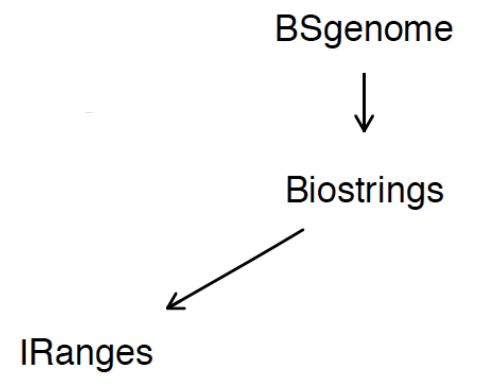
\includegraphics[width=70mm]{diagramas/Seleccio_005.png}
            \end{figure}
  \eit
\end{frame}

%--------------------------------------------------------------------------------------------------------------------------------

\begin{frame}[fragile]
\frametitle{Available genomes}
  \bit
      \item Easy to find out
          \begin{uncoverenv}
\begin{Schunk}
\begin{Sinput}
> require(BSgenome)
> head(available.genomes())
\end{Sinput}
\begin{Soutput}
[1] "BSgenome.Alyrata.JGI.v1"                
[2] "BSgenome.Amellifera.BeeBase.assembly4"  
[3] "BSgenome.Amellifera.UCSC.apiMel2"       
[4] "BSgenome.Amellifera.UCSC.apiMel2.masked"
[5] "BSgenome.Athaliana.TAIR.04232008"       
[6] "BSgenome.Athaliana.TAIR.TAIR9"          
\end{Soutput}
\end{Schunk}
          \end{uncoverenv}
      \item However, large genomes(i.e. human, mouse, ... ) packages might take log to transfer.
  \eit
\end{frame}

%--------------------------------------------------------------------------------------------------------------------------------

\begin{frame}[fragile]
\frametitle{BSgenome Class overview (c'ed)}
  \begin{columns}
  \begin{column}[t]{0.45\textwidth}%
  \bit
      \item Important:
        \bit
            \item proper S4 class usage ban accessing a slot through the ``@'' accessor, except within a package scope.
            \item Hence, it is nowhere to be seen on the present slide
        \eit
  \eit
  \end{column}
    
  \begin{column}[t]{0.45\textwidth}%
        \begin{uncoverenv}
\begin{Schunk}
\begin{Sinput}
> library(BSgenome.Dmelanogaster.UCSC.dm3)
> # Dmelanogaster@seqs_dir
> #Dmelanogaster@masks_dir    ERROR
> #dir(Dmelanogaster@masks_dir)
\end{Sinput}
\end{Schunk}
        \end{uncoverenv}
  \end{column}
  \end{columns}
\end{frame}

%--------------------------------------------------------------------------------------------------------------------------------

\begin{frame}
\frametitle{BSgenome methods}
  \bit
      \item \textbf{Sequence selection}: $[[,\$ $
      \item \textbf{Subsequence selection}: getSeq
      \item \textbf{Accesors}: length, names/seqnames, mseqnames, seqlengths, masknames, sourceUrl
      \item \textbf{Matching}: all Biostings methods
      \item \textbf{SNPs}: injectSNPs, SNPlocs_pkgname,SNPcount, SNPlocs
  \eit
\end{frame}

%--------------------------------------------------------------------------------------------------------------------------------

\begin{frame}[fragile]
\frametitle{Sequence information}
  \bit
      \item operation that do not load sequences
        \begin{uncoverenv}
\begin{Schunk}
\begin{Sinput}
> require(BSgenome.Dmelanogaster.UCSC.dm3)
> head(seqnames(Dmelanogaster))
\end{Sinput}
\begin{Soutput}
[1] "chr2L" "chr2R" "chr3L" "chr3R" "chr4"  "chrX" 
\end{Soutput}
\begin{Sinput}
> head(seqlengths(Dmelanogaster))
\end{Sinput}
\begin{Soutput}
   chr2L    chr2R    chr3L    chr3R     chr4     chrX 
23011544 21146708 24543557 27905053  1351857 22422827 
\end{Soutput}
\end{Schunk}
        \end{uncoverenv}
      \item operation that do
        \begin{uncoverenv}
\begin{Schunk}
\begin{Sinput}
> alphabetFrequency(Dmelanogaster[["chr4"]],baseOnly=TRUE)
\end{Sinput}
\begin{Soutput}
     A      C      G      T  other 
430227 238155 242039 441336    100 
\end{Soutput}
\end{Schunk}
        \end{uncoverenv}      
  \eit
\end{frame}

%--------------------------------------------------------------------------------------------------------------------------------

\begin{frame}[fragile]
\frametitle{Masked vs unmasked}
  \begin{column}[t]{1\textwidth}%
  \bit
      \item unmasked package
        \bit
            \item e.g Dmelanogaster
        \eit
      \item masked packages
        \bit
            \item e.g Hsapiens
        \eit
  \eit
        \begin{uncoverenv}
\begin{Schunk}
\begin{Sinput}
> library(BSgenome.Hsapiens.UCSC.hg19)
> Hsapiens[["chr1"]]
\end{Sinput}
\begin{Soutput}
  249250621-letter "DNAString" instance
seq: NNNNNNNNNNNNNNNNNNNNNNNNNNNNNNNNNNNN...NNNNNNNNNNNNNNNNNNNNNNNNNNNNNNNNNNNN
\end{Soutput}
\end{Schunk}
        \end{uncoverenv}   
  \end{column}
\end{frame}

%--------------------------------------------------------------------------------------------------------------------------------

\begin{frame}[fragile]
\frametitle{Extending Biostrings. Example 1}
  \bit
      \item Applying the Biostrings matching functions:
         \begin{uncoverenv}
\begin{Schunk}
\begin{Sinput}
> exclude<-setdiff(seqnames(Hsapiens),c("chr1","chr2"))
> vcountPattern("ACYTANCAGT", Hsapiens, fixed=c(pattern=FALSE, subject=TRUE), exclude=exclude)
\end{Sinput}
\begin{Soutput}
  seqname strand count
1    chr1      +  1546
2    chr1      -  1545
3    chr2      +  1722
4    chr2      -  1684
\end{Soutput}
\begin{Sinput}
> #vmatchPattern("ACYTANCAGT",Hsapiens, fixed=c(pattern=FALSE, subject=TRUE), exclude=exclude, 
> #asRangedData=FALSE)
\end{Sinput}
\end{Schunk}
        \end{uncoverenv}   
  \eit
\end{frame}

%--------------------------------------------------------------------------------------------------------------------------------

\begin{frame}[fragile]
\frametitle{Example 2}
  \begin{column}[t]{1\textwidth}%
          \bit
              \item Using a Pattern Dictionary, e.g. a library of microarray probes
          \eit
        \begin{uncoverenv}
\begin{Schunk}
\begin{Sinput}
> library(hgu95av2probe)
> probes<-DNAStringSet(hgu95av2probe$sequence[1:100])
> probes[1:10]
\end{Sinput}
\begin{Soutput}
  A DNAStringSet instance of length 10
     width seq
 [1]    25 TGGCTCCTGCTGAGGTCCCCTTTCC
 [2]    25 GGCTGTGAATTCCTGTACATATTTC
 [3]    25 GCTTCAATTCCATTATGTTTTAATG
 [4]    25 GCCGTTTGACAGAGCATGCTCTGCG
 [5]    25 TGACAGAGCATGCTCTGCGTTGTTG
 [6]    25 CTCTGCGTTGTTGGTTTCACCAGCT
 [7]    25 GGTTTCACCAGCTTCTGCCCTCACA
 [8]    25 TTCTGCCCTCACATGCACAGGGATT
 [9]    25 CCTCACATGCACAGGGATTTAACAA
[10]    25 TCCTTGGTACTCTGCCCTCCTGTCA
\end{Soutput}
\end{Schunk}
        \end{uncoverenv}   
  \end{column}
\end{frame}
%--------------------------------------------------------------------------------------------------------------------------------
\begin{frame}[fragile]
\frametitle{Example 2}
  \begin{column}[t]{1\textwidth}%
        \begin{uncoverenv}
\begin{Schunk}
\begin{Sinput}
> counts<-vcountPDict(probes,Hsapiens,exclude=exclude);counts
\end{Sinput}
\begin{Soutput}
DataFrame with 400 rows and 4 columns
    seqname strand     index count
      <Rle>  <Rle> <integer> <Rle>
1      chr1      +         1     0
2      chr1      +         2     0
3      chr1      +         3     0
4      chr1      +         4     0
5      chr1      +         5     0
...     ...    ...       ...   ...
396    chr2      -        96     0
397    chr2      -        97     0
398    chr2      -        98     0
399    chr2      -        99     0
400    chr2      -       100     0
\end{Soutput}
\begin{Sinput}
> #whichMatch<-seqselect(counts$index,counts$count>0);whichMatch  No existeix seqselect!!
> #matchedProbes<- probes[WhichMatch];matchedProbes
> #matchLocs<-matchPDict(PDict(matchedProbes),Hsapiens$chr2);matchLocs
> #extractAllMatches(Hsapiens$chr2,matchLocs)
\end{Sinput}
\end{Schunk}
        \end{uncoverenv}   
  \end{column}
\end{frame}

%--------------------------------------------------------------------------------------------------------------------------------

\begin{frame}[fragile]
\frametitle{Example 5}
  \bit
      \item A new interesting feature is the possibility to inject SNPs!
  \eit
        \begin{column}[t]{0.45\textwidth}%
        \begin{uncoverenv}
\begin{Schunk}
\begin{Sinput}
> cat(available.SNPs(),sep="\n")
\end{Sinput}
\begin{Soutput}
SNPlocs.Hsapiens.dbSNP.20090506
SNPlocs.Hsapiens.dbSNP.20100427
SNPlocs.Hsapiens.dbSNP.20101109
SNPlocs.Hsapiens.dbSNP.20110815
SNPlocs.Hsapiens.dbSNP.20111119
SNPlocs.Hsapiens.dbSNP.20120608
\end{Soutput}
\begin{Sinput}
> library("SNPlocs.Hsapiens.dbSNP.20090506")
> HsWithSNPs<-injectSNPs(Hsapiens,
+           "SNPlocs.Hsapiens.dbSNP.20090506")
> 
> 
\end{Sinput}
\end{Schunk}
        \end{uncoverenv}   
        \end{column}
\end{frame}

%--------------------------------------------------------------------------------------------------------------------------------
\begin{frame}[fragile]
\frametitle{Example 5}
\begin{column}[t]{1\textwidth}%
        \begin{uncoverenv}
\begin{Schunk}
\begin{Sinput}
> HsWithSNPs
\end{Sinput}
\begin{Soutput}
Human genome
| 
| organism: Homo sapiens (Human)
| provider: UCSC
| provider version: hg19
| release date: Feb. 2009
| release name: Genome Reference Consortium GRCh37
| with SNPs injected from package: SNPlocs.Hsapiens.dbSNP.20090506
| 
| single sequences (see '?seqnames'):
|   chr1                   chr2                   chr3                 
|   chr4                   chr5                   chr6                 
|   chr7                   chr8                   chr9                 
|   chr10                  chr11                  chr12                
|   chr13                  chr14                  chr15                
|   chr16                  chr17                  chr18                
|   chr19                  chr20                  chr21                
|   chr22                  chrX                   chrY                 
|   chrM                   chr1_gl000191_random   chr1_gl000192_random 
|   chr4_ctg9_hap1         chr4_gl000193_random   chr4_gl000194_random 
|   chr6_apd_hap1          chr6_cox_hap2          chr6_dbb_hap3        
|   chr6_mann_hap4         chr6_mcf_hap5          chr6_qbl_hap6        
|   chr6_ssto_hap7         chr7_gl000195_random   chr8_gl000196_random 
|   chr8_gl000197_random   chr9_gl000198_random   chr9_gl000199_random 
|   chr9_gl000200_random   chr9_gl000201_random   chr11_gl000202_random
|   chr17_ctg5_hap1        chr17_gl000203_random  chr17_gl000204_random
|   chr17_gl000205_random  chr17_gl000206_random  chr18_gl000207_random
|   chr19_gl000208_random  chr19_gl000209_random  chr21_gl000210_random
|   chrUn_gl000211         chrUn_gl000212         chrUn_gl000213       
|   chrUn_gl000214         chrUn_gl000215         chrUn_gl000216       
|   chrUn_gl000217         chrUn_gl000218         chrUn_gl000219       
|   chrUn_gl000220         chrUn_gl000221         chrUn_gl000222       
|   chrUn_gl000223         chrUn_gl000224         chrUn_gl000225       
|   chrUn_gl000226         chrUn_gl000227         chrUn_gl000228       
|   chrUn_gl000229         chrUn_gl000230         chrUn_gl000231       
|   chrUn_gl000232         chrUn_gl000233         chrUn_gl000234       
|   chrUn_gl000235         chrUn_gl000236         chrUn_gl000237       
|   chrUn_gl000238         chrUn_gl000239         chrUn_gl000240       
|   chrUn_gl000241         chrUn_gl000242         chrUn_gl000243       
|   chrUn_gl000244         chrUn_gl000245         chrUn_gl000246       
|   chrUn_gl000247         chrUn_gl000248         chrUn_gl000249       
| 
| multiple sequences (see '?mseqnames'):
|   upstream1000  upstream2000  upstream5000  
| 
| (use the '$' or '[[' operator to access a given sequence)
\end{Soutput}
\begin{Sinput}
> #SNPlocs_pkgname(HsWithSNPs)
> #SNPcount(HsWithSNPs)
> #alphabetFrequency(Hsapiens$chr1)
> #alphabetFrequency(HsWithSNPs$chr1)
\end{Sinput}
\end{Schunk}
        \end{uncoverenv}   
        \end{column}
\end{frame}
%--------------------------------------------------------------------------------------------------------------------------------

\begin{frame}[fragile]
\frametitle{What next?}
\begin{column}{1\textwidth}
  \bit
      \item Now that we can acces genomic information, it would be useful to import the related annotation. That's (one of) the purpose of the following packages:
        \bit
            \item \textbf{rtracklayer}
            \item \textbf{GenomicFeatures}
            \item \textbf{biomaRt}
            \item \textbf{genomeIntervals}
        \eit
      \item \textbf{rtracklayer} offers export function too and as alredy presented, \textbf{genomeIntervals} offers interval utilities similar to \textbf{IRanges}
  \eit
\end{column}
\end{frame}

%--------------------------------------------------------------------------------------------------------------------------------

\begin{frame}
\frametitle{rtracklayer}
    \begin{figure}[ht]
    \centering
    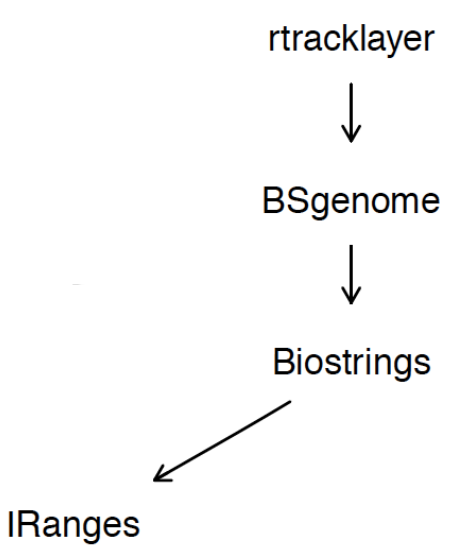
\includegraphics[width=60mm]{diagramas/Seleccio_006.png}
    \end{figure}
\end{frame}

%--------------------------------------------------------------------------------------------------------------------------------

\begin{frame}
\frametitle{Methods}
\begin{column}{1\textwidth}
  \bit
      \item There are two high level methods 
        \bit
            \item import
            \item export
        \eit
      \item Both accept the following formats:
        \bit
            \item BED: bed, bedGraph, bed15
            \item GFF: gff1, 2 and 3
            \item WIG
        \eit
      \item export works with \emph{RangedData} objects
      \item import returns a \emph{RangedData} object or \emph{GRanges} object, depending on the (asRangedData) boolean argument.
  \eit
\end{column}
\end{frame}

%--------------------------------------------------------------------------------------------------------------------------------

\begin{frame}
\frametitle{Methods (c'ed)}
\begin{column}{1\textwidth}
  \bit
      \item When exporting
        \bit
            \item The naming convention of the \emph{RangedData} column names is crucial.
            \item The following column names 
              \bit
                  \item \textbf{names}: for exporting the feature names
                  \item \textbf{scores}: for exporting the feature scores
                  \item \textbf{strand}: for exporting the feature strands
                  \item \textbf{see} ?export.bed for the complete  details
              \eit
        \eit
  \eit
  \end{column}
\end{frame}

%--------------------------------------------------------------------------------------------------------------------------------

\begin{frame}
\frametitle{GenomicFeatures}
\begin{column}{1\textwidth}
  \bit
      \item manegement of transcript information
        \bit
            \item using \textbf{GenomicRanges}
            \item stored into SQLite databases
        \eit
      \begin{figure}[ht]
      \centering
      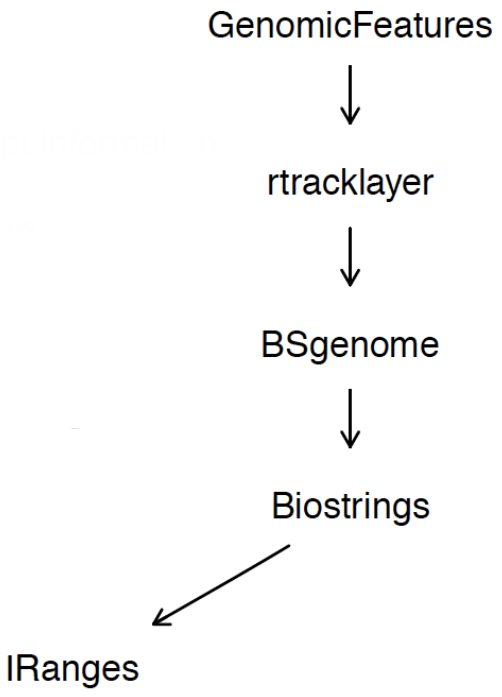
\includegraphics[width=40mm]{diagramas/Seleccio_007.png}
      \end{figure}
  \eit
  \end{column}
\end{frame}

%--------------------------------------------------------------------------------------------------------------------------------

\begin{frame}[fragile]
\frametitle{Constructors and Class}
  \bit
      \item makeTranscriptDbFromBiomart
      \item makeTrascriptDbFromUCSC
          \begin{uncoverenv}
\begin{Schunk}
\begin{Sinput}
> library(GenomicFeatures)
> head(supportedUCSCtables())
\end{Sinput}
\begin{Soutput}
                       track           subtrack
knownGene         UCSC Genes               <NA>
knownGeneOld3 Old UCSC Genes               <NA>
ccdsGene                CCDS               <NA>
refGene         RefSeq Genes               <NA>
xenoRefGene     Other RefSeq               <NA>
vegaGene          Vega Genes Vega Protein Genes
\end{Soutput}
\begin{Sinput}
> mm9KG<-makeTranscriptDbFromUCSC(genome="mm9",tablename="knownGene")
> saveFeatures(mm9KG,file="mm9KG.sqlite")
\end{Sinput}
\end{Schunk}
          \end{uncoverenv}   
  \eit
\end{frame}

%--------------------------------------------------------------------------------------------------------------------------------
\begin{frame}[fragile]
\frametitle{Constructors and Class}
          \begin{uncoverenv}
\begin{Schunk}
\begin{Sinput}
> mm9KG<-loadFeatures("mm9KG.sqlite")
> mm9KG
\end{Sinput}
\begin{Soutput}
TranscriptDb object:
| Db type: TranscriptDb
| Supporting package: GenomicFeatures
| Data source: UCSC
| Genome: mm9
| Organism: Mus musculus
| UCSC Table: knownGene
| Resource URL: http://genome.ucsc.edu/
| Type of Gene ID: Entrez Gene ID
| Full dataset: yes
| miRBase build ID: NA
| transcript_nrow: 55419
| exon_nrow: 246570
| cds_nrow: 213117
| Db created by: GenomicFeatures package from Bioconductor
| Creation time: 2014-06-07 22:03:43 +0200 (Sat, 07 Jun 2014)
| GenomicFeatures version at creation time: 1.16.2
| RSQLite version at creation time: 0.11.4
| DBSCHEMAVERSION: 1.0
\end{Soutput}
\end{Schunk}
          \end{uncoverenv}   
\end{frame}
%--------------------------------------------------------------------------------------------------------------------------------

\begin{frame}
\frametitle{Extractors}
\begin{column}{1\textwidth}
  \bit
      \item ungrouped
        \bit
            \item transcriptBy
            \item exonsBy
            \item intronsByTranscript
            \item fiveUTRsByTranscript
            \item threeUTRsByTranscript
        \eit
  \eit
\end{column}
\end{frame}
  
%--------------------------------------------------------------------------------------------------------------------------------
\begin{frame}[fragile]
\frametitle{Extractors}
     \begin{uncoverenv}
\begin{Schunk}
\begin{Sinput}
> library(GenomicFeatures)
> txExons<-exonsBy(mm9KG)
> head(txExons)
\end{Sinput}
\begin{Soutput}
GRangesList of length 6:
$1 
GRanges with 8 ranges and 3 metadata columns:
      seqnames             ranges strand |   exon_id   exon_name exon_rank
         <Rle>          <IRanges>  <Rle> | <integer> <character> <integer>
  [1]     chr1 [4797974, 4798063]      + |         1        <NA>         1
  [2]     chr1 [4798536, 4798567]      + |         2        <NA>         2
  [3]     chr1 [4818665, 4818730]      + |         3        <NA>         3
  [4]     chr1 [4820349, 4820396]      + |         4        <NA>         4
  [5]     chr1 [4822392, 4822462]      + |         5        <NA>         5
  [6]     chr1 [4827082, 4827155]      + |         6        <NA>         6
  [7]     chr1 [4829468, 4829569]      + |         7        <NA>         7
  [8]     chr1 [4831037, 4832908]      + |         9        <NA>         8

$2 
GRanges with 9 ranges and 3 metadata columns:
      seqnames             ranges strand | exon_id exon_name exon_rank
  [1]     chr1 [4797974, 4798063]      + |       1      <NA>         1
  [2]     chr1 [4798536, 4798567]      + |       2      <NA>         2
  [3]     chr1 [4818665, 4818730]      + |       3      <NA>         3
  [4]     chr1 [4820349, 4820396]      + |       4      <NA>         4
  [5]     chr1 [4822392, 4822462]      + |       5      <NA>         5
  [6]     chr1 [4827082, 4827155]      + |       6      <NA>         6
  [7]     chr1 [4829468, 4829569]      + |       7      <NA>         7
  [8]     chr1 [4831037, 4831213]      + |       8      <NA>         8
  [9]     chr1 [4835044, 4836816]      + |      10      <NA>         9

...
<4 more elements>
---
seqlengths:
         chr1         chr2         chr3 ...  chrY_random chrUn_random
    197195432    181748087    159599783 ...     58682461      5900358
\end{Soutput}
\begin{Sinput}
> 
\end{Sinput}
\end{Schunk}
      \end{uncoverenv}   
\end{frame}
  



%--------------------------------------------------------------------------------------------------------------------------------

\begin{frame}
\frametitle{Usage}
\begin{column}{1\textwidth}
  \bit
      \item Overlapping with transcripts
        \bit
            \item findOverlaps
            \item countOverlaps
            \item match
            \item \%in\%
            \item subsetByOverlaps
        \eit
      \item More about these in the following part about \textbf{GenomicRanges}
  \eit
\end{column}
\end{frame}

%--------------------------------------------------------------------------------------------------------------------------------

\begin{frame}
\frametitle{biomaRt}
\begin{column}{1\textwidth}
  \bit
      \item Side note to get help from within R:
        \bit
            \item vignette(``biomaRt'',package=``biomaRt'')
        \eit
      \item biomaRt is an interface to the collection of databases that implements the bioMart software suite:
        \bit
            \item \url{http://biomart.org}
            \item allow retrieval og huge datasets from different sources through a common interface
            \item examples are: Ensembl, HapMap, Uniprot, ...
        \eit        
  \eit
\end{column}
\end{frame}

%--------------------------------------------------------------------------------------------------------------------------------

\begin{frame}[fragile]
\frametitle{biomaRt, an example}
\begin{column}{1\textwidth}
  \bit
      \item Connect the mart database
          \begin{uncoverenv}
\begin{Schunk}
\begin{Sinput}
> require(biomaRt)
> ensembl<- useMart("ensembl")
> head(listDatasets(ensembl))
\end{Sinput}
\begin{Soutput}
                         dataset                                description
1         oanatinus_gene_ensembl     Ornithorhynchus anatinus genes (OANA5)
2        cporcellus_gene_ensembl            Cavia porcellus genes (cavPor3)
3        gaculeatus_gene_ensembl     Gasterosteus aculeatus genes (BROADS1)
4         lafricana_gene_ensembl         Loxodonta africana genes (loxAfr3)
5 itridecemlineatus_gene_ensembl Ictidomys tridecemlineatus genes (spetri2)
6        choffmanni_gene_ensembl        Choloepus hoffmanni genes (choHof1)
  version
1   OANA5
2 cavPor3
3 BROADS1
4 loxAfr3
5 spetri2
6 choHof1
\end{Soutput}
\begin{Sinput}
> ensembl<- useMart("ensembl",dataset="dmelanogaster_gene_ensembl")
> head(listAttributes(ensembl))
\end{Sinput}
\begin{Soutput}
                   name           description
1       ensembl_gene_id       Ensembl Gene ID
2 ensembl_transcript_id Ensembl Transcript ID
3    ensembl_peptide_id    Ensembl Protein ID
4       ensembl_exon_id       Ensembl Exon ID
5           description           Description
6       chromosome_name       Chromosome Name
\end{Soutput}
\end{Schunk}
          \end{uncoverenv}   
  \eit
\end{column}
\end{frame}

%--------------------------------------------------------------------------------------------------------------------------------

\begin{frame}[fragile]
\frametitle{biomaRt, an example (c'ed)}
\begin{column}{1\textwidth}
  \bit
      \item   query the database
          \begin{uncoverenv}
\begin{Schunk}
\begin{Sinput}
> exon.annotation<-getBM(c("ensemb_gene_id","strand",
+                 "chromosome_name","ensembl_exon_id",
+                 "exon_chrom_start","exon_chrom_end"),
+                 mart=ensembl,filters="chromosome_name",
+                 values="4")
\end{Sinput}
\end{Schunk}
          \end{uncoverenv}   
    \item convert into a RangedData / Granges
  \eit
\end{column}
\end{frame}

%--------------------------------------------------------------------------------------------------------------------------------

\begin{frame}
\frametitle{genomeIntervals}
\begin{column}{1\textwidth}
  \bit
      \item   Similar interval implementation to IRanges
        \bit
            \item (+) overall faster, gff function more robust to 'incorrect' format
            \item (-) less integrated in R
        \eit
      \item Two classes:
        \bit
            \item Genome\_intervals
            \item Genome\_intervals\_stranded
        \eit
      \item Methods
        \bit
            \item input
              \bit
                  \item \textbf{ readGff3, getGffAttributes}, parseGffAttributes
              \eit
            \item intervals utilities
              \bit
                  \item interval\_overlap, \textbf{interval\_complement}, interval\_union, interval\_intersection
              \eit
        \eit
  \eit
\end{column}
\end{frame}

%--------------------------------------------------------------------------------------------------------------------------------

\begin{frame}
\frametitle{What next?}
\begin{column}{1\textwidth}
  \bit
      \item We have seen how to get genomic sequences and their annotation
      \item For processing NGS data, we are now missing the other half of the workflow: loading and manipulating the actual data. For this, three packages are available.
        \bit
            \item \textbf{GenomicRanges}
            \item \textbf{Rsamtools}
            \item \textbf{ShortRead}
        \eit
  \eit
\end{column}
\end{frame}

%--------------------------------------------------------------------------------------------------------------------------------

\begin{frame}
\frametitle{GenomicRanges}
\begin{column}{1\textwidth}
    \begin{figure}[ht]
    \centering
    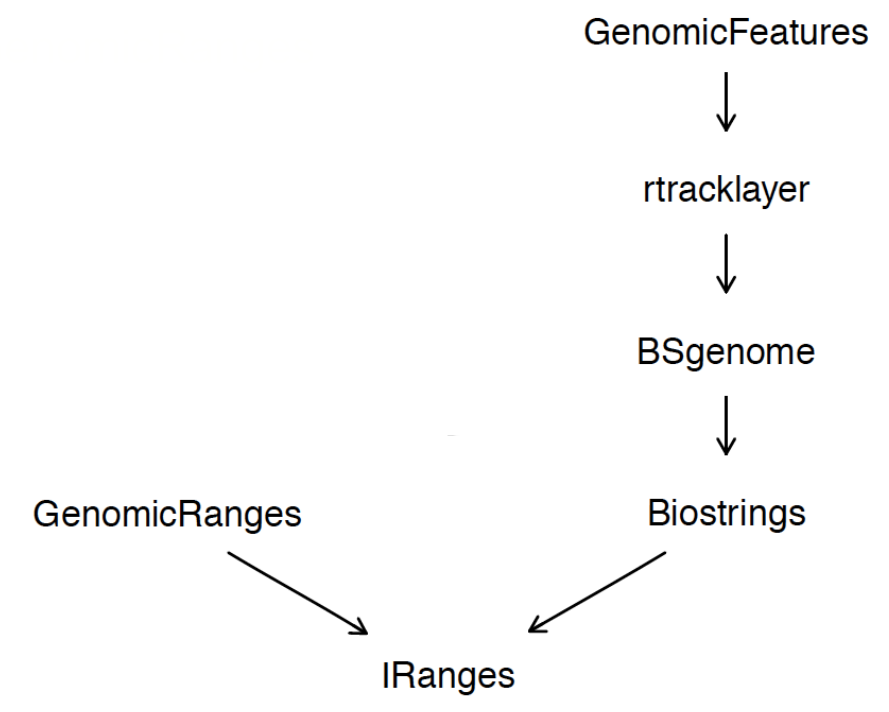
\includegraphics[width=80mm]{diagramas/Seleccio_008.png}
    \end{figure}
\end{column}
\end{frame}

%--------------------------------------------------------------------------------------------------------------------------------

\begin{frame}
\frametitle{Naive approach}
\begin{column}{1\textwidth}
  \bit
      \item   Genomic coordinates consist of
        \bit
            \item chromosome 
            \item position
            \item strand
            \item additional information
              \bit
                  \item GC content
                  \item etc.
              \eit
        \eit
      \item This caan be represented by a data.frame
        \bit
            \item fine for organism information ($\sim$ 100k exons, 20k genes)
            \item not for million of reads 
        \eit
  \eit
\end{column}
\end{frame}

%--------------------------------------------------------------------------------------------------------------------------------

\begin{frame}
\frametitle{BIOC representation for intervals with data}
\begin{column}{1\textwidth}
  \bit
      \item \emph{RangedData}
        \bit
            \item used by \textbf{rtracklayer}
            \item interval grouped by chromosome/conting
            \item strand unaware
        \eit
      \item \emph{GRanges}
        \bit
          \item used by \textbf{GenomicFeatures}
          \item intervals not required to be grouped by chromosome/contig
          \item strand aware
          \item \emph{GRangesList} can hold exons with spliced transcripts 
        \eit
  \eit
\end{column}
\end{frame}

%--------------------------------------------------------------------------------------------------------------------------------

\begin{frame}[fragile]
\frametitle{GRanges constructor and slots}
\begin{column}{1\textwidth}
  \bit
      \item starts and ends defined in an \emph{IRanges} object
      \item strand, seqnames (chromosome) and seqlenghts (chromosome size) to be provided
          \begin{uncoverenv}
\begin{Schunk}
\begin{Sinput}
> grngs<-GRanges(seqnames=c("chr1","chr2","chr1"), 
+       ranges=IRanges(start=c(3,4,1),end=c(7,5,3)),
+     strand=c("+","+","-"),seqlengths = c("chr1"=24,"chr2"=18))
> grngs
\end{Sinput}
\begin{Soutput}
GRanges with 3 ranges and 0 metadata columns:
      seqnames    ranges strand
         <Rle> <IRanges>  <Rle>
  [1]     chr1    [3, 7]      +
  [2]     chr2    [4, 5]      +
  [3]     chr1    [1, 3]      -
  ---
  seqlengths:
   chr1 chr2
     24   18
\end{Soutput}
\end{Schunk}
          \end{uncoverenv}   
      \item additional slots can contain mtadata information
          \begin{uncoverenv}
\begin{Schunk}
\begin{Sinput}
> getSlots("GRanges")
\end{Sinput}
\begin{Soutput}
       seqnames          ranges          strand elementMetadata         seqinfo 
          "Rle"       "IRanges"           "Rle"     "DataFrame"       "Seqinfo" 
       metadata 
         "list" 
\end{Soutput}
\end{Schunk}
          \end{uncoverenv}  
  \eit
\end{column}
\end{frame}

%--------------------------------------------------------------------------------------------------------------------------------

\begin{frame}
\frametitle{Interval operations}
\begin{column}{1\textwidth}
  \bit
      \item Intra-interval
        \bit
            \item flank,resize,shift
        \eit
      \item Inter-interval
        \bit
            \item disjoin, gaps, reduce, range
            \item coverage
        \eit
      \item Between intervals sets
        \bit
            \item union, intersect, setdiff
            \item punion,pintersectm psetdiff
            \item findOverlaps, countOverlaps, \%in\%, match
        \eit
      \item Low Level
        \bit
            \item start,end,width
        \eit
  \eit
  \end{column}
\end{frame}

%--------------------------------------------------------------------------------------------------------------------------------

\begin{frame}[fragile]
\frametitle{Other functions}
\begin{column}{1\textwidth}
  \bit
      \item Selecting
        \bit
            \item seqselect, [
            \item head, tail, window
            \item subset, subsetByOverlaps
                     \begin{uncoverenv}
\begin{Schunk}
\begin{Sinput}
> grngs[strand(grngs)== "-"]
\end{Sinput}
\begin{Soutput}
GRanges with 1 range and 0 metadata columns:
      seqnames    ranges strand
         <Rle> <IRanges>  <Rle>
  [1]     chr1    [1, 3]      -
  ---
  seqlengths:
   chr1 chr2
     24   18
\end{Soutput}
\begin{Sinput}
> # seqselect(grngs,strand(grngs)=="-") NO EXISTEIX seqselect
\end{Sinput}
\end{Schunk}
        \end{uncoverenv}  
        \eit
  \eit
  \end{column}
\end{frame}

%--------------------------------------------------------------------------------------------------------------------------------

\begin{frame}[fragile]
\frametitle{Example 1: Intra-interval}
\begin{columns}

\begin{column}{0.45\textwidth}
  \bit
      \item shift
           \begin{uncoverenv}
\begin{Schunk}
\begin{Sinput}
> grngs
\end{Sinput}
\begin{Soutput}
GRanges with 3 ranges and 0 metadata columns:
      seqnames    ranges strand
         <Rle> <IRanges>  <Rle>
  [1]     chr1    [3, 7]      +
  [2]     chr2    [4, 5]      +
  [3]     chr1    [1, 3]      -
  ---
  seqlengths:
   chr1 chr2
     24   18
\end{Soutput}
\begin{Sinput}
> shift(grngs,1)
\end{Sinput}
\begin{Soutput}
GRanges with 3 ranges and 0 metadata columns:
      seqnames    ranges strand
         <Rle> <IRanges>  <Rle>
  [1]     chr1    [4, 8]      +
  [2]     chr2    [5, 6]      +
  [3]     chr1    [2, 4]      -
  ---
  seqlengths:
   chr1 chr2
     24   18
\end{Soutput}
\end{Schunk}
        \end{uncoverenv}  
  \eit
  \end{column}
  
  \begin{column}{0.55\textwidth}
  \bit
      \item resize
           \begin{uncoverenv}
\begin{Schunk}
\begin{Sinput}
> resize(grngs,10)
\end{Sinput}
\begin{Soutput}
GRanges with 3 ranges and 0 metadata columns:
      seqnames    ranges strand
         <Rle> <IRanges>  <Rle>
  [1]     chr1   [3, 12]      +
  [2]     chr2   [4, 13]      +
  [3]     chr1   [1,  3]      -
  ---
  seqlengths:
   chr1 chr2
     24   18
\end{Soutput}
\end{Schunk}
        \end{uncoverenv} 
      \item flank
           \begin{uncoverenv}
\begin{Schunk}
\begin{Sinput}
> flank(grngs,2)
\end{Sinput}
\begin{Soutput}
GRanges with 3 ranges and 0 metadata columns:
      seqnames    ranges strand
         <Rle> <IRanges>  <Rle>
  [1]     chr1    [1, 2]      +
  [2]     chr2    [2, 3]      +
  [3]     chr1    [4, 5]      -
  ---
  seqlengths:
   chr1 chr2
     24   18
\end{Soutput}
\end{Schunk}
        \end{uncoverenv}  
  \eit
  \end{column}
  
\end{columns}
\end{frame}

%--------------------------------------------------------------------------------------------------------------------------------

\begin{frame}[fragile]
\frametitle{Overlap detection}
\begin{column}{1\textwidth}
  \bit
      \item \emph{findOverlap} and \emph{countOverlaps} produce a mapping and a tabulation of interval overlaps, respectively
            \begin{uncoverenv}
\begin{Schunk}
\begin{Sinput}
> ol<-findOverlaps(grngs,reduce(grngs))
> ol
\end{Sinput}
\begin{Soutput}
Hits of length 3
queryLength: 3
subjectLength: 3
  queryHits subjectHits 
   <integer>   <integer> 
 1         1           1 
 2         2           3 
 3         3           2 
\end{Soutput}
\end{Schunk}
        \end{uncoverenv}       
  \eit
  \end{column}
\end{frame}

%--------------------------------------------------------------------------------------------------------------------------------

\begin{frame}
\frametitle{Rsamtools}
Blue represents the ''+'' strand, red the''-'' strand
 \begin{figure}[ht]
    \centering
    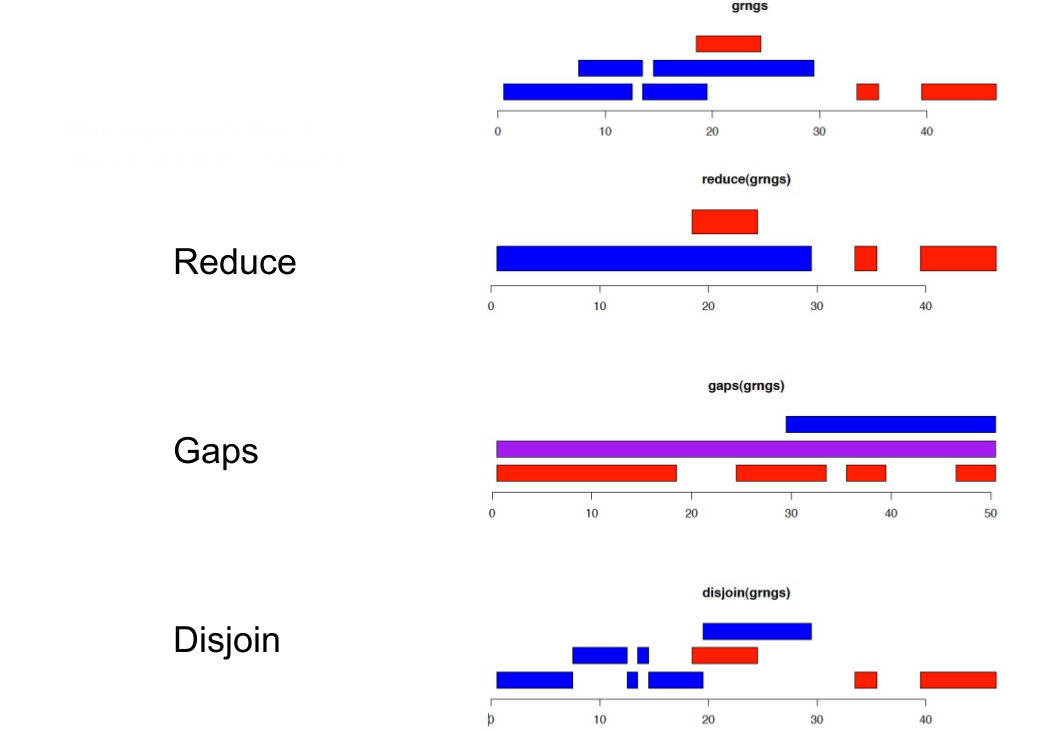
\includegraphics[width=100mm]{diagramas/Seleccio_009.png}
  \end{figure}
\end{frame}

%--------------------------------------------------------------------------------------------------------------------------------

\begin{frame}
\frametitle{samtools and Rsamtools}
\begin{column}{1\textwidth}
  \bit
      \item samtools
        \bit
            \item Data Format: SAM(text) and BAM (binary)
            \item Tools: merge, sort, pileup, view, etc.
        \eit
      \item Rsamtools
        \bit
            \item Reads and represents BAMfiles
            \item high level: readAligned (type=BAM), readPileup
            \item lower level: scanBam, scanBamParam, ScanBamWhat
            \item utilities: countBam, sortBam, indexBam, filterBam, scanBamHeader
            \item views: BamViews
        \eit
  \eit
  \end{column}
\end{frame}

%--------------------------------------------------------------------------------------------------------------------------------

\begin{frame}[fragile]
\frametitle{Input}
\begin{column}{1\textwidth}
  \bit
      \item   \small{readAligned} returns an \emph{alignedRead} class
        \bit
            \item described in the following section on \textbf{ShortRead}
        \eit
      \item \small{scanBam} returns a list of list i.e.. one list per column in the SAM file.
        \bit
            \item qname: a \emph{BStringSet} containing the read id 
            \item seq: a \emph{DNAStringSet} containing the read sequence
            \item etc.
            \item The possible fields can be found with \small{scanBamWhat()}
              \begin{uncoverenv}
\begin{Schunk}
\begin{Sinput}
> require(Rsamtools)
> scanBamWhat()
\end{Sinput}
\begin{Soutput}
 [1] "qname"       "flag"        "rname"       "strand"      "pos"        
 [6] "qwidth"      "mapq"        "cigar"       "mrnm"        "mpos"       
[11] "isize"       "seq"         "qual"        "groupid"     "mate_status"
\end{Soutput}
\end{Schunk}
        \end{uncoverenv}    
        \eit
      \item \small{scanBam} is the function called by the \textbf{GenomicRanges} \small{readGappedAlignments} method
  \eit
  \end{column}
\end{frame}

%--------------------------------------------------------------------------------------------------------------------------------

\begin{frame}[fragile]
\frametitle{Input (c'ed)}
\begin{column}{1\textwidth}
  \bit
      \item   The input can be controlled using \small{ScanBamParam}
        \bit
            \item it has three fields
              \bit
                  \item \textbf{which}: \emph{GRanges} selecting references, genomic loci, strand, ...
                    
                  \item \textbf{flag}: use the SAM flag to selected paired, mapped, etc. reads.
                        \begin{uncoverenv}
\begin{Schunk}
\begin{Sinput}
> names(formals(scanBamFlag))
\end{Sinput}
\begin{Soutput}
 [1] "isPaired"                    "isProperPair"               
 [3] "isUnmappedQuery"             "hasUnmappedMate"            
 [5] "isMinusStrand"               "isMateMinusStrand"          
 [7] "isFirstMateRead"             "isSecondMateRead"           
 [9] "isNotPrimaryRead"            "isNotPassingQualityControls"
[11] "isDuplicate"                 "isValidVendorRead"          
\end{Soutput}
\end{Schunk}
                        \end{uncoverenv}    
                  \item \textbf{what}: fields to retrieve (cf. \small{scanBamWhat})
              \eit
        \eit
  \eit
  \end{column}
\end{frame}

%--------------------------------------------------------------------------------------------------------------------------------

\begin{frame}
\frametitle{GappedAlignments vs AlignedRead}
\begin{column}{1\textwidth}
  \bit
      \item \emph{AlignedRead}
        \bit
            \item reads complete files
            \item include sequence, quality, identifier, etc.
            \item reads are assumed to be ungapped
        \eit
      \item \emph{GappedAlignments}
        \bit
            \item use scanBam
            \item genomic coordinates, 'cigar', covered intervals
            \item Cigar: an RLE; M(match), I (insertion), D (deleiton), N (skipped), P (padding), S/H (soft/hard clip)
            \item direct IRanges accesors (sub-setting, narrowing, coverage)
        \eit
  \eit
  \end{column}
\end{frame}

%--------------------------------------------------------------------------------------------------------------------------------

\begin{frame}
\frametitle{BamViews}
\begin{column}{1\textwidth}
  \bit
      \item Acces a set of experiments stored in BAM files
        \bit
            \item for example to query a specific loci
        \eit 
      \item Check the vignette ("leeViews")
      \item Still very unstable!
  \eit
  \end{column}
  
\end{frame}

%--------------------------------------------------------------------------------------------------------------------------------

\begin{frame}[fragile]
\frametitle{BamViews}
  \begin{column}{1.3\textwidth}
                        \begin{uncoverenv}
\begin{Schunk}
\begin{Sinput}
> library(leeBamViews)
> bpaths=dir(system.file("bam",package="leeBamViews"),full=TRUE, patt="bam$")
> gt<- do.call(rbind, strsplit(basename(bpaths),"_"))[,1]
> geno<-substr(gt,1,nchar(gt)-1)
> lane<- substr(gt,nchar(gt),nchar(gt))
> pd=DataFrame(geno=geno, lane=lane, row.names=paste(geno,lane,sep="."))
> bs1=BamViews(bamPaths=bpaths, bamSamples=pd, bamExperiment=list(annotation="org.Sc.sgd.db"))
> bamPaths(bs1)
\end{Sinput}
\begin{Soutput}
                                                                      isowt.5 
"/home/alex/R/x86_64-pc-linux-gnu-library/3.1/leeBamViews/bam/isowt5_13e.bam" 
                                                                      isowt.6 
"/home/alex/R/x86_64-pc-linux-gnu-library/3.1/leeBamViews/bam/isowt6_13e.bam" 
                                                                        rlp.5 
  "/home/alex/R/x86_64-pc-linux-gnu-library/3.1/leeBamViews/bam/rlp5_13e.bam" 
                                                                        rlp.6 
  "/home/alex/R/x86_64-pc-linux-gnu-library/3.1/leeBamViews/bam/rlp6_13e.bam" 
                                                                        ssr.1 
  "/home/alex/R/x86_64-pc-linux-gnu-library/3.1/leeBamViews/bam/ssr1_13e.bam" 
                                                                        ssr.2 
  "/home/alex/R/x86_64-pc-linux-gnu-library/3.1/leeBamViews/bam/ssr2_13e.bam" 
                                                                        xrn.1 
  "/home/alex/R/x86_64-pc-linux-gnu-library/3.1/leeBamViews/bam/xrn1_13e.bam" 
                                                                        xrn.2 
  "/home/alex/R/x86_64-pc-linux-gnu-library/3.1/leeBamViews/bam/xrn2_13e.bam" 
\end{Soutput}
\end{Schunk}
                        \end{uncoverenv}    
  \end{column}
\end{frame}

%--------------------------------------------------------------------------------------------------------------------------------
\begin{frame}[fragile]
\frametitle{BamViews}
  \begin{column}{1.3\textwidth}
                        \begin{uncoverenv}
\begin{Schunk}
\begin{Sinput}
> bamSamples(bs1)
\end{Sinput}
\begin{Soutput}
DataFrame with 8 rows and 2 columns
               geno        lane
        <character> <character>
isowt.5       isowt           5
isowt.6       isowt           6
rlp.5           rlp           5
rlp.6           rlp           6
ssr.1           ssr           1
ssr.2           ssr           2
xrn.1           xrn           1
xrn.2           xrn           2
\end{Soutput}
\begin{Sinput}
> sel<-GRanges(seqnames="Scchr13",IRanges(start=861250,end=863000),strand="+")
> # covex=RleList(lapply(bamPaths(bs1),function(x) coverage(readGappedAlignments(x))[[1]]))
\end{Sinput}
\end{Schunk}
                        \end{uncoverenv}    
  \end{column}
\end{frame}


%--------------------------------------------------------------------------------------------------------------------------------

\begin{frame}
\frametitle{ShortRead}
\begin{column}{1\textwidth}
      \begin{figure}[ht]
      \centering
      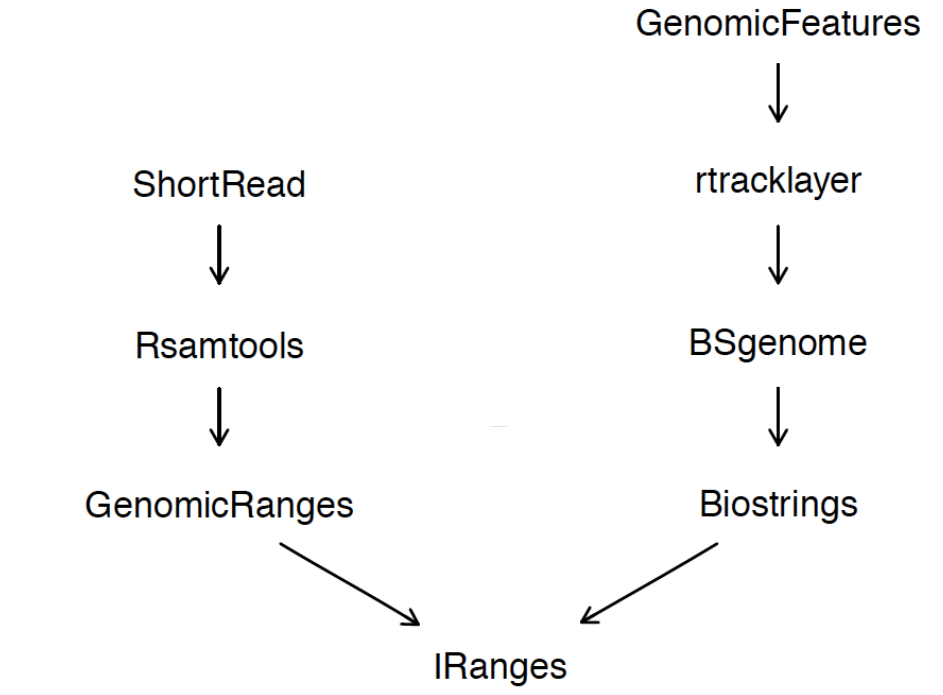
\includegraphics[width=90mm]{diagramas/Seleccio_011.png}
      \end{figure}
  \end{column}
\end{frame}

%--------------------------------------------------------------------------------------------------------------------------------

\begin{frame}
\frametitle{ShortRead}
\begin{column}{1\textwidth}
  \bit
      \item Input
        \bit
            \item read most sequence proprietary formats
            \item read fastq
            \item read BAM
        \eit
      \item Exploration
        \bit
            \item contains sequence, quality, id, etc. information
        \eit
      \item Manipulation
        \bit
            \item allow the manipulation of the fields with a limited memory impact
        \eit
      \item Quality assessment
        \bit
            \item offers quality assessment functionalities
        \eit
  \eit
  \end{column}
\end{frame}

%--------------------------------------------------------------------------------------------------------------------------------

\begin{frame}[fragile]
\frametitle{AlignedReadClass}
\begin{column}{1\textwidth}
  \bit
      \item   The main class to store the read information
                     \begin{uncoverenv}
\begin{Schunk}
\begin{Sinput}
> require(ShortRead)
> showClass("AlignedRead")
\end{Sinput}
\begin{Soutput}
Class "AlignedRead" [package "ShortRead"]

Slots:
                                                                          
Name:        chromosome         position           strand     alignQuality
Class:           factor          integer           factor     QualityScore
                                                                          
Name:         alignData          quality            sread               id
Class: AlignedDataFrame     QualityScore     DNAStringSet       BStringSet

Extends: 
Class "ShortReadQ", directly
Class "ShortRead", by class "ShortReadQ", distance 2
Class ".ShortReadBase", by class "ShortReadQ", distance 3
\end{Soutput}
\end{Schunk}
                        \end{uncoverenv}  
      \item All slots can be accessed through accordingly named accessors
  \eit
  \end{column}
\end{frame}

%--------------------------------------------------------------------------------------------------------------------------------

\begin{frame} [fragile]
\frametitle{SRFilterclass}
\begin{column}{1\textwidth}
  \bit
      \item \small{Useful tools to filter the reads during or after the import}
      \begin{uncoverenv}
\begin{Schunk}
\begin{Sinput}
> showClass("SRFilter")
\end{Sinput}
\begin{Soutput}
Class "SRFilter" [package "ShortRead"]

Slots:
                                      
Name:            .Data            name
Class:        function ScalarCharacter

Extends: 
Class "function", from data part
Class ".SRUtil", directly
Class "OptionalFunction", by class "function", distance 2
Class "PossibleMethod", by class "function", distance 2
Class "expressionORfunction", by class "function", distance 2
Class "functionORNULL", by class "function", distance 2
\end{Soutput}
\end{Schunk}
       \end{uncoverenv}  
       \item \small{many already implemented}
        \bit
            \item \tiny{idFilter}
            \item \tiny{chromosomeFilter}
            \item \tiny{positionFilter}
            \item \tiny{strandFilter}
            \item \tiny{etc.}
        \eit
      \item \small{They can be combined using compose}
        \bit
            \item \small{compose(idFilter,chromosomeFilter)}
        \eit
  \eit
  \end{column}
\end{frame}

%--------------------------------------------------------------------------------------------------------------------------------

\begin{frame}[fragile]
\frametitle{Other classes}
\begin{column}{1\textwidth}
  \bit
      \item The package implements many classes to hold the different kind of data
            \begin{uncoverenv}
\begin{Schunk}
\begin{Sinput}
> getClasses(where="package:ShortRead")
\end{Sinput}
\begin{Soutput}
 [1] "AlignedDataFrame"       "AlignedRead"            "ArrayIntensity"        
 [4] "BAMQA"                  "BowtieQA"               "ExperimentPath"        
 [7] "FastqFile"              "FastqFileList"          "FastqFileReader"       
[10] "FastqQA"                "FastqQuality"           "FastqSampler"          
[13] "FastqSamplerList"       "FastqStreamer"          "FastqStreamerList"     
[16] "IntegerQuality"         "Intensity"              "IntensityInfo"         
[19] "IntensityMeasure"       "MAQMapQA"               "MatrixQuality"         
[22] "NumericQuality"         "QA"                     ".QA"                   
[25] ".QA2"                   "QAAdapterContamination" "QACollate"             
[28] "QAData"                 "QAFastqSource"          "QAFiltered"            
[31] "QAFlagged"              "QAFrequentSequence"     "QANucleotideByCycle"   
[34] "QANucleotideUse"        "QAQualityByCycle"       "QAQualityUse"          
[37] "QAReadQuality"          "QASequenceUse"          "QASource"              
[40] "QASummary"              "QualityScore"           ".Roche"                
[43] "RochePath"              "RocheSet"               "RtaIntensity"          
[46] "SFastqQuality"          "ShortRead"              ".ShortReadBase"        
[49] "ShortReadFile"          "ShortReadQ"             "ShortReadQQA"          
[52] "Snapshot"               "SnapshotFunction"       "SnapshotFunctionList"  
[55] ".Solexa"                "SolexaExportQA"         "SolexaIntensity"       
[58] "SolexaIntensityInfo"    "SolexaPath"             "SolexaRealignQA"       
[61] "SolexaSet"              "SpTrellis"              "SRError"               
[64] "SRFilter"               "SRFilterResult"         "SRList"                
[67] "SRSet"                  ".SRUtil"                "SRVector"              
[70] "SRWarn"                 "trellis"               
\end{Soutput}
\end{Schunk}
       \end{uncoverenv} 
  \eit
  \end{column}
\end{frame}

%--------------------------------------------------------------------------------------------------------------------------------

\begin{frame}[fragile]
\frametitle{Input and accessor examples}
\begin{column}{1\textwidth}
  \bit
      \item Simple walk through
            \begin{uncoverenv}
\begin{Schunk}
\begin{Sinput}
> require("EatonEtAlChIPseq")
> fl<-system.file("extdata","GSM424494_wt_G2_orc_chip_rep1_S288C_14.mapview.txt.gz",package="EatonEtAlChIPseq")
> aln<-readAligned(fl,type="MAQMapview");aln
\end{Sinput}
\begin{Soutput}
class: AlignedRead
length: 478774 reads; width: 39 cycles
chromosome: S288C_14 S288C_14 ... S288C_14 S288C_14 
position: 2 4 ... 784295 784295 
strand: + - ... + + 
alignQuality: IntegerQuality 
alignData varLabels: nMismatchBestHit mismatchQuality nExactMatch24 nOneMismatch24 
\end{Soutput}
\begin{Sinput}
> head(sread(aln))
\end{Sinput}
\begin{Soutput}
  A DNAStringSet instance of length 6
    width seq
[1]    39 CGGCTTTCTGACCGAAATTAAAAAAAAAAAATGAAAATG
[2]    39 GATTTATGAAAGAAATTAAAAAAAAAAAATGAAAATGAA
[3]    39 CTTTCTGACCGAAATTAAAAAAAAAAAATGAAAATGAAA
[4]    39 TTTCTGACCGAAATTAAAAAAAAAAAATGAAATTGAAAC
[5]    39 TTTATGAAAGAAAATAAAAAAAAAAAATGAAAATGAAAC
[6]    39 TTTCTGAAAGAAATTAAAAAAAAAAAATGAAAATGAAAC
\end{Soutput}
\end{Schunk}
       \end{uncoverenv} 
  \eit
  \end{column}
\end{frame}

%--------------------------------------------------------------------------------------------------------------------------------

\begin{frame}[fragile]
\frametitle{Input and accessor examples}
\begin{column}{1\textwidth}
  \bit
       \item with filters
                   \begin{uncoverenv}
\begin{Schunk}
\begin{Sinput}
> filter<- compose(chromosomeFilter("S288C_14"),positionFilter(min=1,max=1000))
> alnF<-readAligned(fl,type="MAQMapview",filter=filter);alnF
\end{Sinput}
\begin{Soutput}
class: AlignedRead
length: 715 reads; width: 39 cycles
chromosome: S288C_14 S288C_14 ... S288C_14 S288C_14 
position: 2 4 ... 997 999 
strand: + - ... - - 
alignQuality: IntegerQuality 
alignData varLabels: nMismatchBestHit mismatchQuality nExactMatch24 nOneMismatch24 
\end{Soutput}
\end{Schunk}
       \end{uncoverenv} 
  \eit
  \end{column}
\end{frame}

%--------------------------------------------------------------------------------------------------------------------------------


\begin{frame}[fragile]
\frametitle{Input and accessor examples}
\begin{column}{1\textwidth}
      \begin{uncoverenv}
\begin{Schunk}
\begin{Sinput}
> head(quality(aln))
\end{Sinput}
\begin{Soutput}
class: FastqQuality
quality:
  A BStringSet instance of length 6
    width seq
[1]    39 >>>>>>>>>><>>><<<>>5><<><<<<<<44444///,
[2]    39 ,%//4&/14&&:<<<.<>>>>>>>>>>>>>>>>>>>>>>
[3]    39 >>>>>>>>>>>>>>>><><>><>>><<<<<44444////
[4]    39 <>>>>>:<<><::>><>:><<<>><::::<44%-4//$/
[5]    39 ,,/,1+41+4<<<4<<>>>>>>>>>>>>>>>>>>>>>>>
[6]    39 ,++(*44*/<<<<+><>>>>>>>>>>><>>>>>>>>>>>
\end{Soutput}
\begin{Sinput}
> head(id(aln))
\end{Sinput}
\begin{Soutput}
  A BStringSet instance of length 6
    width seq
[1]    23 X8193_200:5:175:690:668
[2]    22 X8193_200:5:62:612:145
[3]    23 X8193_200:5:206:446:786
[4]    22 X8193_200:5:12:950:859
[5]    23 X8193_200:5:230:400:822
[6]    23 X8193_200:5:258:160:889
\end{Soutput}
\end{Schunk}
       \end{uncoverenv} 
  \end{column}
\end{frame}

%--------------------------------------------------------------------------------------------------------------------------------

\begin{frame}[fragile]
\frametitle{Manipulation example}
\begin{column}{1\textwidth}
  \bit
      \item For example to rename chromosome
      \begin{uncoverenv}
\begin{Schunk}
\begin{Sinput}
> chrom<-chromosome(alnF)
> i<-sub("S288C_([[:digit:]]+)","\\1",levels(chrom));i
\end{Sinput}
\begin{Soutput}
[1] "14"
\end{Soutput}
\begin{Sinput}
> levels(chrom)
\end{Sinput}
\begin{Soutput}
[1] "S288C_14"
\end{Soutput}
\begin{Sinput}
> levels(chrom)<-paste("chr",as.roman(i),sep="")
> levels(chrom)
\end{Sinput}
\begin{Soutput}
[1] "chrXIV"
\end{Soutput}
\begin{Sinput}
> alnF<-renew(alnF,chromosome=chrom);alnF
\end{Sinput}
\begin{Soutput}
class: AlignedRead
length: 715 reads; width: 39 cycles
chromosome: chrXIV chrXIV ... chrXIV chrXIV 
position: 2 4 ... 997 999 
strand: + - ... - - 
alignQuality: IntegerQuality 
alignData varLabels: nMismatchBestHit mismatchQuality nExactMatch24 nOneMismatch24 
\end{Soutput}
\begin{Sinput}
> 
\end{Sinput}
\end{Schunk}
       \end{uncoverenv} 
  \eit
  \end{column}
\end{frame}

%--------------------------------------------------------------------------------------------------------------------------------


\begin{frame}[fragile]
\frametitle{Quality assessment}
\begin{columns}
\begin{column}{0.3\textwidth}
  \bit
      \item Many functions are available in \textbf{ShortRead} that can be used for performing QA
      \begin{uncoverenv}
\begin{Schunk}
\begin{Sinput}
> f.list<-showMethods(
+ where="package:ShortRead",
+ printTo=FALSE)
\end{Sinput}
\end{Schunk}
       \end{uncoverenv}   
       \vspace{8cm}
  \eit
  \end{column}
  
  \begin{column}{0.65\textwidth}
      \begin{uncoverenv}
\begin{Schunk}
\begin{Sinput}
> sapply(strsplit(f.list[grep("Function",f.list)],' '),
+        function(x)x[2])
\end{Sinput}
\begin{Soutput}
  [1] "alphabet"                      "alphabetByCycle"              
  [3] "alphabetFrequency"             "alphabetScore"                
  [5] "annTrack"                      "append"                       
  [7] "!"                             "["                            
  [9] "[["                            "$<-"                          
 [11] "$"                             "c"                            
 [13] "chromosome"                    "clean"                        
 [15] "coerce"                        "to=\"classGeneratorFunction\""
 [17] "to=\"OptionalFunction\""       "to=\"genericFunction\""       
 [19] "to=\"OptionalFunction\""       "to=\"genericFunction\""       
 [21] "countLines"                    "coverage"                     
 [23] "dim"                           "dustyScore"                   
 [25] "encoding"                      "experimentPath"               
 [27] "fac"                           "FastqFileList"                
 [29] "FastqQuality"                  "FastqSamplerList"             
 [31] "FastqStreamerList"             "FastqStreamer"                
 [33] "files"                         "flag"                         
 [35] "functions"                     "getTrellis"                   
 [37] "id"                            "ignore.strand"                
 [39] "%in%"                          "laneNames"                    
 [41] "lapply"                        "length"                       
 [43] "names<-"                       "names"                        
 [45] "name"                          "narrow"                       
 [47] "pan"                           "pData"                        
 [49] "phenoData"                     "position"                     
 [51] "qa2"                           "QACollate"                    
 [53] "qa"                            "rbind"                        
 [55] "read454"                       "readAligned"                  
 [57] "readBaseQuality"               "readFastaQual"                
 [59] "readFasta"                     "readFastq"                    
 [61] "readIntensities"               "readPrb"                      
 [63] "readQseq"                      "readQual"                     
 [65] "renewable"                     "renew"                        
 [67] "report_html"                   "report"                       
 [69] "restore"                       "RocheSet"                     
 [71] "runNames"                      "sapply"                       
 [73] "SFastqQuality"                 "ShortReadQ"                   
 [75] "ShortRead"                     "show"                         
 [77] NA                              NA                             
 [79] NA                              NA                             
 [81] NA                              "SnapshotFunctionList"         
 [83] NA                              "Snapshot"                     
 [85] "SolexaSet"                     "srdistance"                   
 [87] "srduplicated"                  "sread"                        
 [89] "srFilter"                      "srorder"                      
 [91] "srrank"                        "srsort"                       
 [93] "stats"                         "strand"                       
 [95] "tables"                        "togglefun"                    
 [97] "togglep"                       "togglez"                      
 [99] "trimEnds"                      "trimLRPatterns"               
[101] "trimTails"                     "trimTailw"                    
[103] "varLabels"                     "varMetadata"                  
[105] "view"                          "vrange"                       
[107] "width"                         "writeFasta"                   
[109] "writeFastq"                    "yield"                        
[111] "zi"                            "zoom"                         
[113] "zo"                           
\end{Soutput}
\end{Schunk}
       \end{uncoverenv} 
  \end{column}
  \end{columns}
\end{frame}

%--------------------------------------------------------------------------------------------------------------------------------

\begin{frame}[fragile]
\frametitle{QA example (yet another one...)}
\begin{column}{1\textwidth}
  \bit
      \item   Using independent functions
      \begin{uncoverenv}
\begin{Schunk}
\begin{Sinput}
> abc<- alphabetByCycle(sread(alnF))
> abc[1:4,1:12]
\end{Sinput}
\begin{Soutput}
        cycle
alphabet [,1] [,2] [,3] [,4] [,5] [,6] [,7] [,8] [,9] [,10] [,11] [,12]
       A  239  246  251  236  244  244  223  207  184   212   217   230
       C  197  172  180  178  169  194  192  194  202   212   185   182
       G  103   88   87  105   89   93  108  101  114    90   103    83
       T  176  209  197  196  213  184  192  213  215   201   210   220
\end{Soutput}
\begin{Sinput}
> abc<-abc[1:4, ]
> par(mfrow=c(1,2))
> matplot(t(abc),type="l",lty=rep(1,4))
> m<-as (quality(alnF),"matrix")
> plot(colMeans(m),type="b")
\end{Sinput}
\end{Schunk}
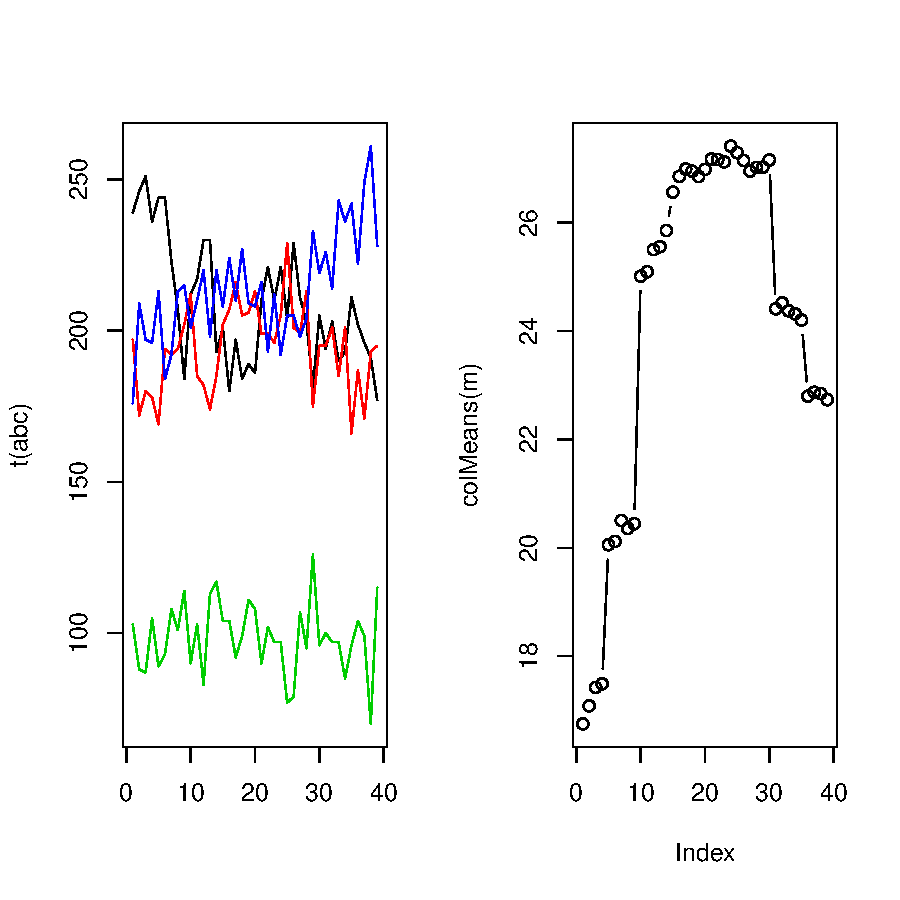
\includegraphics{2.Bioconductor_BLAU-059}
       \end{uncoverenv} 
       \item All these and more are combined into the function: qa()
       \item These can then be reported using the report() function
  \eit
  \end{column}
\end{frame}

%--------------------------------------------------------------------------------------------------------------------------------

\begin{frame}
\frametitle{Conclusion}
\begin{column}{1\textwidth}
      \begin{figure}[ht]
      \centering
      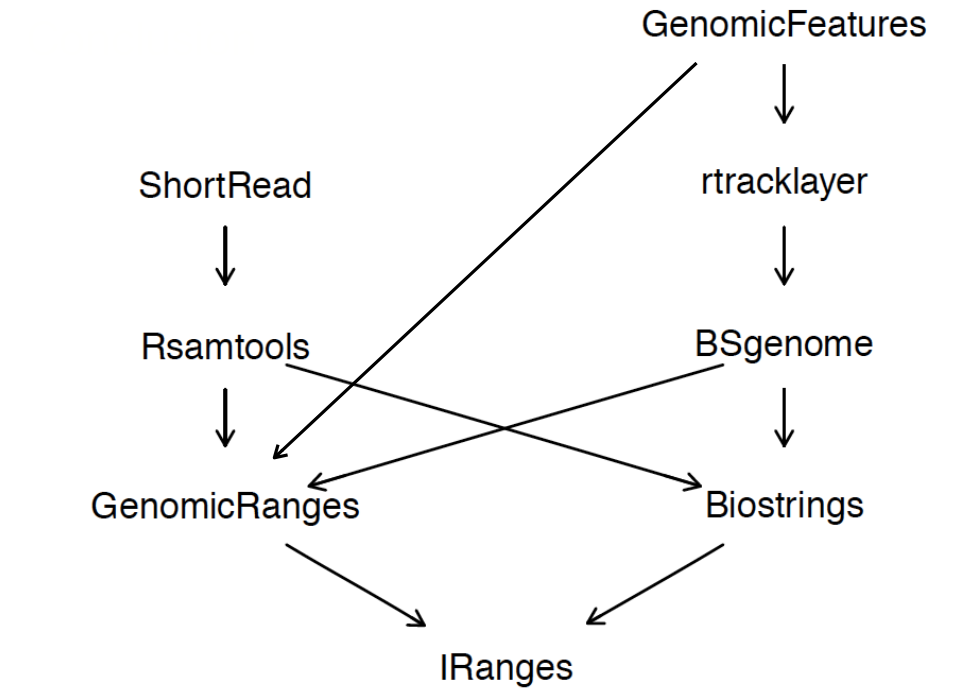
\includegraphics[width=90mm]{diagramas/Seleccio_012.png}
      \end{figure}
  \end{column}
\end{frame}

%--------------------------------------------------------------------------------------------------------------------------------

\begin{frame}
\frametitle{Conclusion}
\begin{column}{1\textwidth}
  \bit
      \item We have seen the two ``branches'' of the core packages:
        \bit
            \item the one used to get genomic sequence and annotation
            \item the one used to load and manipulate NGS data
        \eit
      \item Actually, the cit is not so clear ad the packages of these two branches are interacting at different levels.
      \item They provide numerous functionalities and are getting into a ``production'' (stable development) state.
      \item Higher level packaages are being developed to wrap these functionalities into more user friendly packages.
  \eit
  \end{column}
\end{frame}

%--------------------------------------------------------------------------------------------------------------------------------

\begin{frame}
\frametitle{Conclusion}
\begin{column}{1\textwidth}
  \bit
      \item If you would start today using these packages:
        \bit
            \item go for the BAM format
            \item go for GRanges objects
            \item Be on the lookout, especially for the \emph{SummarizedExperiment} class in the \textbf{GenomicRanges} package.
              \bit
                  \item It is a concept similar to the \emph{ExpressionSet} class devoloped for microarray and aims at normalizing the output of NGS experiments within R/Bioconductor
              \eit
        \eit
  \eit
  \end{column}
\end{frame}

%--------------------------------------------------------------------------------------------------------------------------------

\begin{frame}
\frametitle{If we were fast..}
\begin{column}{1\textwidth}
  \bit
      \item Another couple of package to mention
        \bit
            \item Rsubread (only on linux)
            \item easyRNASeq (self-promotion)
        \eit
  \eit
  \end{column}
\end{frame}

%--------------------------------------------------------------------------------------------------------------------------------

\begin{frame}[fragile]
\frametitle{Rsubread}
\begin{columns}
\begin{column}{0.3\textwidth}
  \bit
      \item a package to align short read in R!
      \item If you have a session on vuori you can try that code slightly modified in the R file to use only chromosome 1
  \eit
  \end{column}
  
\begin{column}{0.6\textwidth}
 \begin{uncoverenv}
\begin{Schunk}
\begin{Sinput}
> ## write the human genome sequences
> writeXStringSet(Reduce(append,
+ lapply(seqnames(Hsapiens),
+ function(nam)
+ {dss<-DNAStringSet(unmasked(Hsapiens[[nam]]))
+ names(dss)<-nam
+ dss})),file="hg19.fa")
> ##create the indexes
> require(Rsubread)
> dir.create("indexes")
> buildindex(basename=file.path("indexes","hg19"),
+            reference="hg19.fa")
> ## align the reads
> sapply(dir(pattern="*\\.gz$"),function(fil){ 
+   ## decomplress the files
+   gunzip(fil)
+   ##align
+   align(index=file.path("indexes","hg19"),
+         readfile1=sub("\\.gz$","",fil),
+         nsubreads=2, TH1=1,
+         output_file=sub("\\.fastq\\.gz$","\\,sam",fil))
+   ## create bam files
+   asBAM(file=sib("\\.fastq\\.gz$","\\.sam",fil),
+         destination=sub("\\.fastq\\.gz$","",fil),
+         indexDestination=TRUE)
+   })
\end{Sinput}
\end{Schunk}
       \end{uncoverenv} 
  \end{column}
\end{columns}
\end{frame}

%--------------------------------------------------------------------------------------------------------------------------------

\begin{frame}
\frametitle{easyRNASeq package}
\begin{column}{0.8\textwidth}
      \begin{figure}[ht]
      \centering
      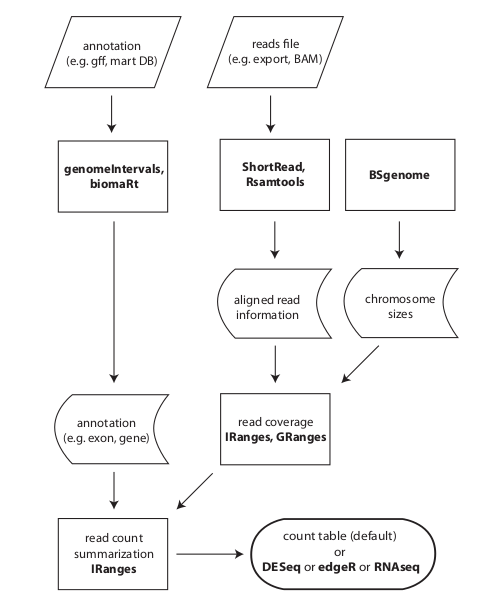
\includegraphics[width=60mm]{diagramas/Seleccio_013.png}
      \end{figure}
  \end{column}
\end{frame}

%--------------------------------------------------------------------------------------------------------------------------------

\begin{frame}
\begin{columns}
\begin{column}{0.6\textwidth}
\frametitle{Replicate comparison}
  \bit
      \item The simplest output is a matrix
        \bit
            \item Comparing replicates is therefore easy
            \item Can be done automatically if the user provides the sample information
            \item GRAFIC
        \eit
  \eit
  \end{column}
\begin{column}{0.6\textwidth}
      \begin{figure}[ht]
      \centering
      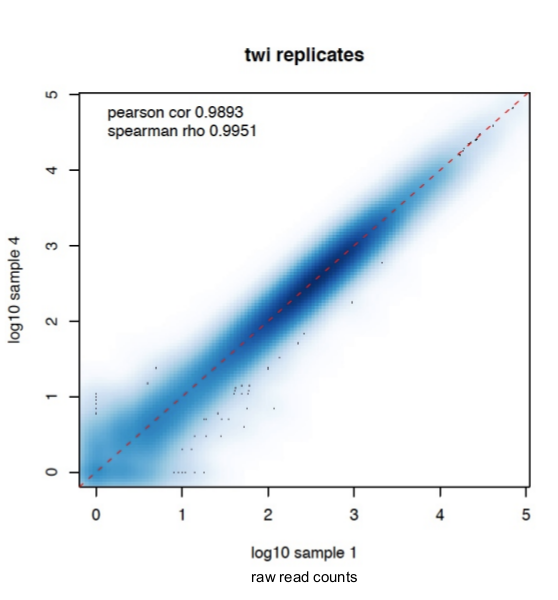
\includegraphics[width=40mm]{diagramas/Seleccio_014.png}
      \end{figure}
\end{column}
\end{columns}
\end{frame}

%--------------------------------------------------------------------------------------------------------------------------------

\begin{frame}
\frametitle{Normalization}
\begin{columns}
\begin{column}{0.6\textwidth}
  \bit
      \item Three types can be applied
        \bit
            \item \textbf{R}eads \textbf{P}er feature \textbf{K}b per \textbf{M}ilion reads in the library
        \eit
      \item DESeq
        \bit
            \item based on Negative Binomial
            \item fit a model to correct for the library sizes
        \eit
      \item edgeR
        \bit
            \item based on Negative Binomial
            \item use a trimmed mean og M-values to correct for the library sizes
        \eit
  \eit
  \end{column}

\begin{column}{0.6\textwidth}
      \begin{figure}[ht]
      \centering
      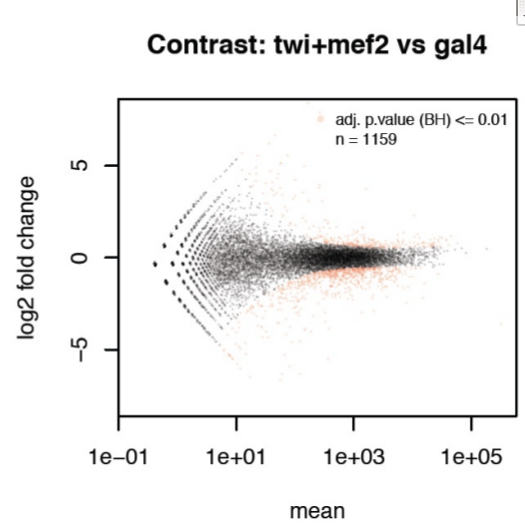
\includegraphics[width=50mm]{diagramas/Seleccio_015.png}
      \end{figure}
\end{column}
\end{columns}
\end{frame}
\end{document}
